\documentclass[12pt]{article}
\usepackage[margin=25mm]{geometry}
\usepackage[utf8]{inputenc}
\usepackage{mathtools}
\usepackage{paralist}
\usepackage{hyperref}
\usepackage{wrapfig}
\usepackage{minted}
\usepackage{helvet}
\usepackage{fnpct}
\usepackage[style=austrian]{csquotes}

\renewcommand{\contentsname}{Inhaltsverzeichnis}
\setminted{fontsize=\small,baselinestretch=1,fontfamily=courier,frame=single}
\setlength\itemsep{-1em}
\linespread{1.5}

\tolerance=1
\emergencystretch=\maxdimen
\hyphenpenalty=10000
\hbadness=10000

\begin{document}
\fontfamily{phv}\fontsize{12pt}{18pt}\selectfont
\thispagestyle{empty}
\begin{center}
\fontsize{20pt}{10pt}\selectfont
Bundesrealgymnasium Keplerstraße Graz, Keplerstraße 1 8020 Graz
\end{center}
\vspace{20mm}
\begin{center}
\fontsize{26pt}{10pt}\selectfont
\textbf{Vorwissenschaftliche Arbeit}
\end{center}
\vspace{20mm}
\begin{center}
\fontsize{28pt}{28pt}\selectfont
\textbf{Entwicklung und Programmierung eines Robotik-Controllerboards basierend auf einem Raspberry Pi in C++}
\end{center}
\vspace{20mm}
\begin{center}
\fontsize{20pt}{32pt}\selectfont
Matteo Valentini\\
8b\\
Betreuerin: Mag.\textsuperscript{a} Nicole Bizjak\\
eingereicht am 10. März 2021
\end{center}

\newpage\section*{Abstract}
Diese Arbeit bildet den gesamten Entwicklungsprozess eines selbstentwickelten Robotik-Controllerboards ab, von der Auswahl der Komponenten, dem Design der Platine bis zur fertigen Programmierschnittstelle, welche in der Programmiersprache C++ geschrieben wurde. Das Resultat ist eine kompakte Platine, welche im Bereich der Robotik für kleinere Roboter eingesetzt werden kann. Das Board ist nicht nur für einen Verwendungszweck abgestimmt, sondern kann in sehr vielen Situation eingesetzt werden. Diese Eigenschaft ergibt sich auf Grund der vielen Schnittstellen sowie der starken Rechenleistung und der Auslegung auf Spannungsbereiche zwischen 7V und 35V. Die dazugehörige Programmierschnittstelle ermöglicht eine Steuerung aller Hardware-Schnittstellen in diversen Modi, sodass ein Großteil möglicher Komponenten ohne großen Programmieraufwand angesteuert werden kann. Jede verbaute Komponente sowie der gesamte Code, welcher für dieses Projekt nötigt ist, werden in dieser Arbeit genau beschrieben und unter die Lupe genommen, damit der Leser sich ein in die Tiefe gehendes Verständnis über den Entwicklungsprozess aneignen kann.
\newpage\tableofcontents
\newpage\section{Einleitung}
Im Jahr 2017 habe ich versucht, eine Plattform mit hoher Rechenleistung für Robotik zu finden und bin dann auf die Bare-Metal-Programmierung von Raspberry Pis gestoßen. Bare Metal bezeichnet hierbei die Programmierung von Systemen, ohne ein Betriebssystem zu verwenden. Nachdem ich mir damals genug Wissen in diesem Bereich angeeignet hatte, begann ich zusätzlich noch mit dem Designen von Leiterplatten, welche anfangs noch auf einer großen Fläche nur wenige Komponenten unterbrachten. In den letzten Jahren lernte ich auch noch SMD-Bauteile mit der Hand zu verlöten, dass das Design von wesentlich kleineren Platinen erlaubte. Auf Grund von diesem Hobby entschloss ich mich dazu, über dieses Thema eine vorwissenschaftliche Arbeit zu verfassen, welche alle Entwicklungsschritte genau dokumentiert.\\\\
Alle Informationen zur Programmierung des Raspberry Pi stammen aus dem offiziellen Datenblatt. Zuerst wird in dieser Arbeit beschrieben, welche Komponenten auf der Platine zu welchen Zwecken verbaut wurden sowie die Besonderheiten, auf jene zu Achten ist. Anschließend wird der Bootprozess des Raspberry Pi erklärt, bevor die Programmierung aller Hardware-Controller erfolgt. Als nächstes wird die Entwicklung der Software für den verbauten Subprozessor, einem ATmega644, beschrieben. Nach der ATmega-Software folgt die Implementierung aller Schnittstellen, die über den ATmega funktionieren, in die C++-Library. Abschließend wird noch beschrieben, wie eigene Komponenten mit dem Board genutzt werden können.
\newpage\section{Hardware}
In diesem Kapitel werden die einzelnen Komponenten sowie die verschiedenen Kommunikationen wie I2C und SPI genauer beschrieben. Zusätzlich dazu werden bestimmte Design-Entscheidungen wie zum Beispiel die Trennung der Spannungsbereiche begründet.
\subsection{Layout und Anschlüsse}
Die Platine hat eine Größe von 69 * 85.5mm, da dies die kleinstmögliche Größe war, auf der alle Komponenten untergebracht werden konnten. Die beiden Kupferschichten haben jeweils eine Stärke von 1 oz und sind bestmöglich verwendet, sodass alle Leiterbahnen gezogen werden konnten.\\\\
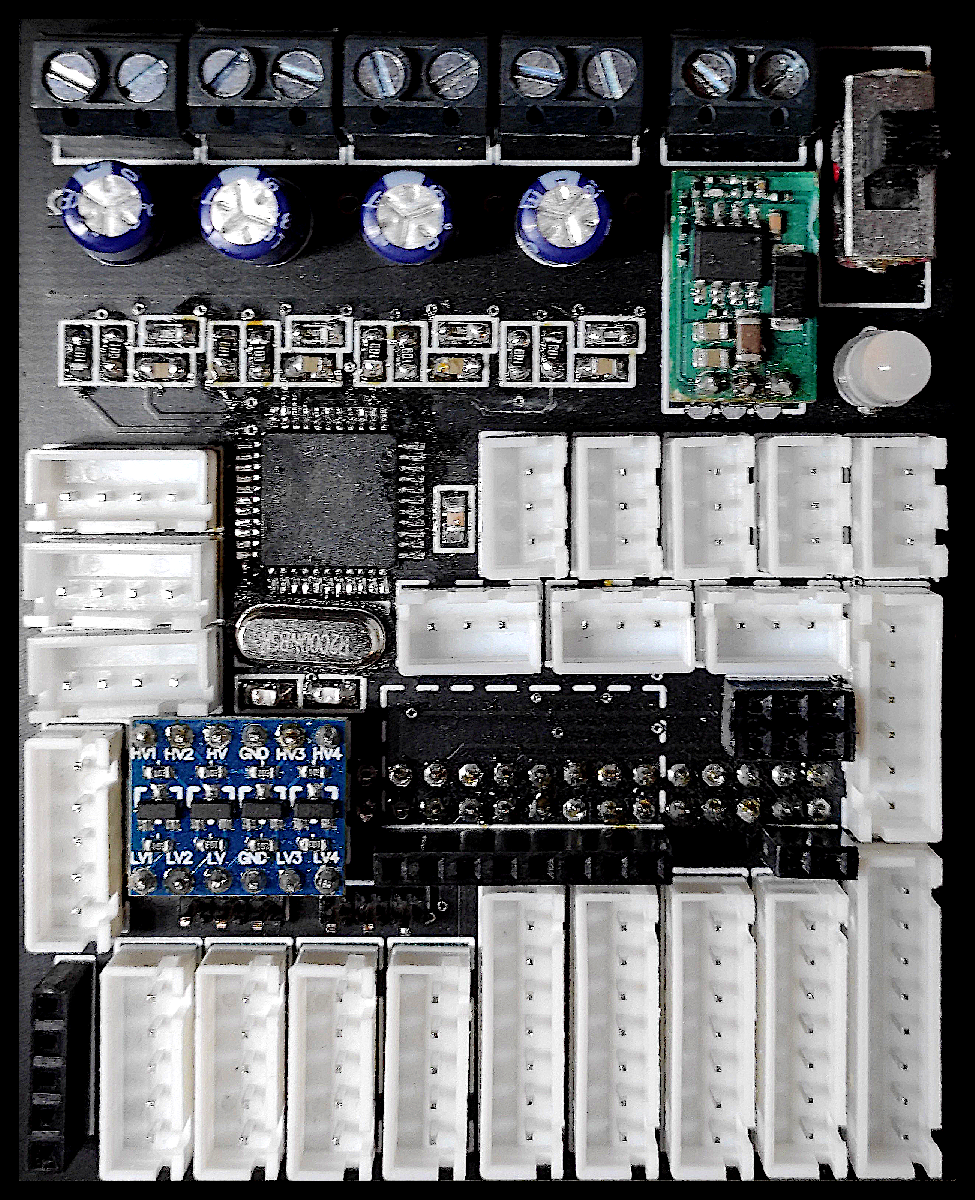
\includegraphics[width=0.49\textwidth]{img/vwa1.png}
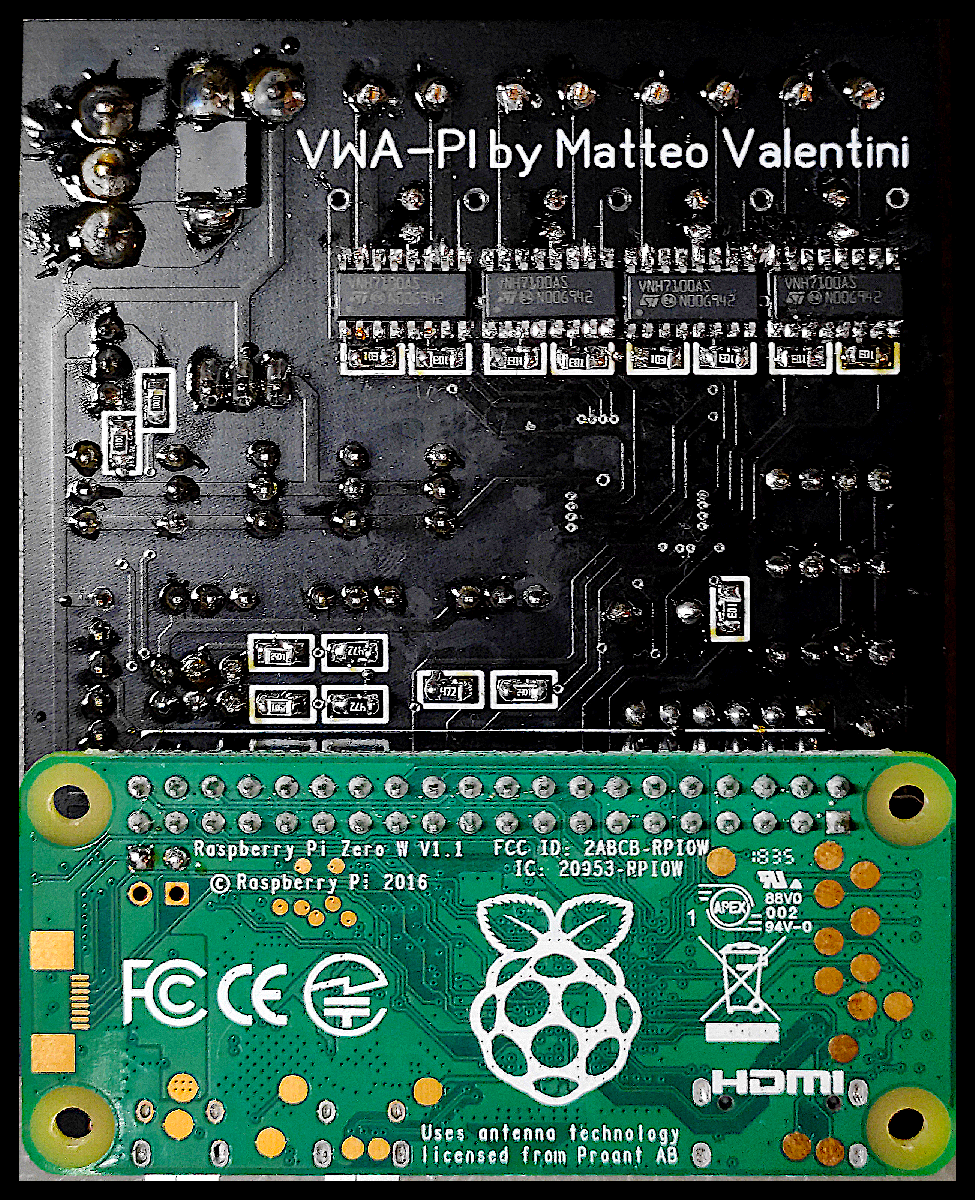
\includegraphics[width=0.49\textwidth]{img/vwa2.png}
\begin{center}\raisebox{8mm}{Abbildung 1: Ansicht der fertig bestückten Platine von oben und unten (Foto: Verf.)}\end{center}
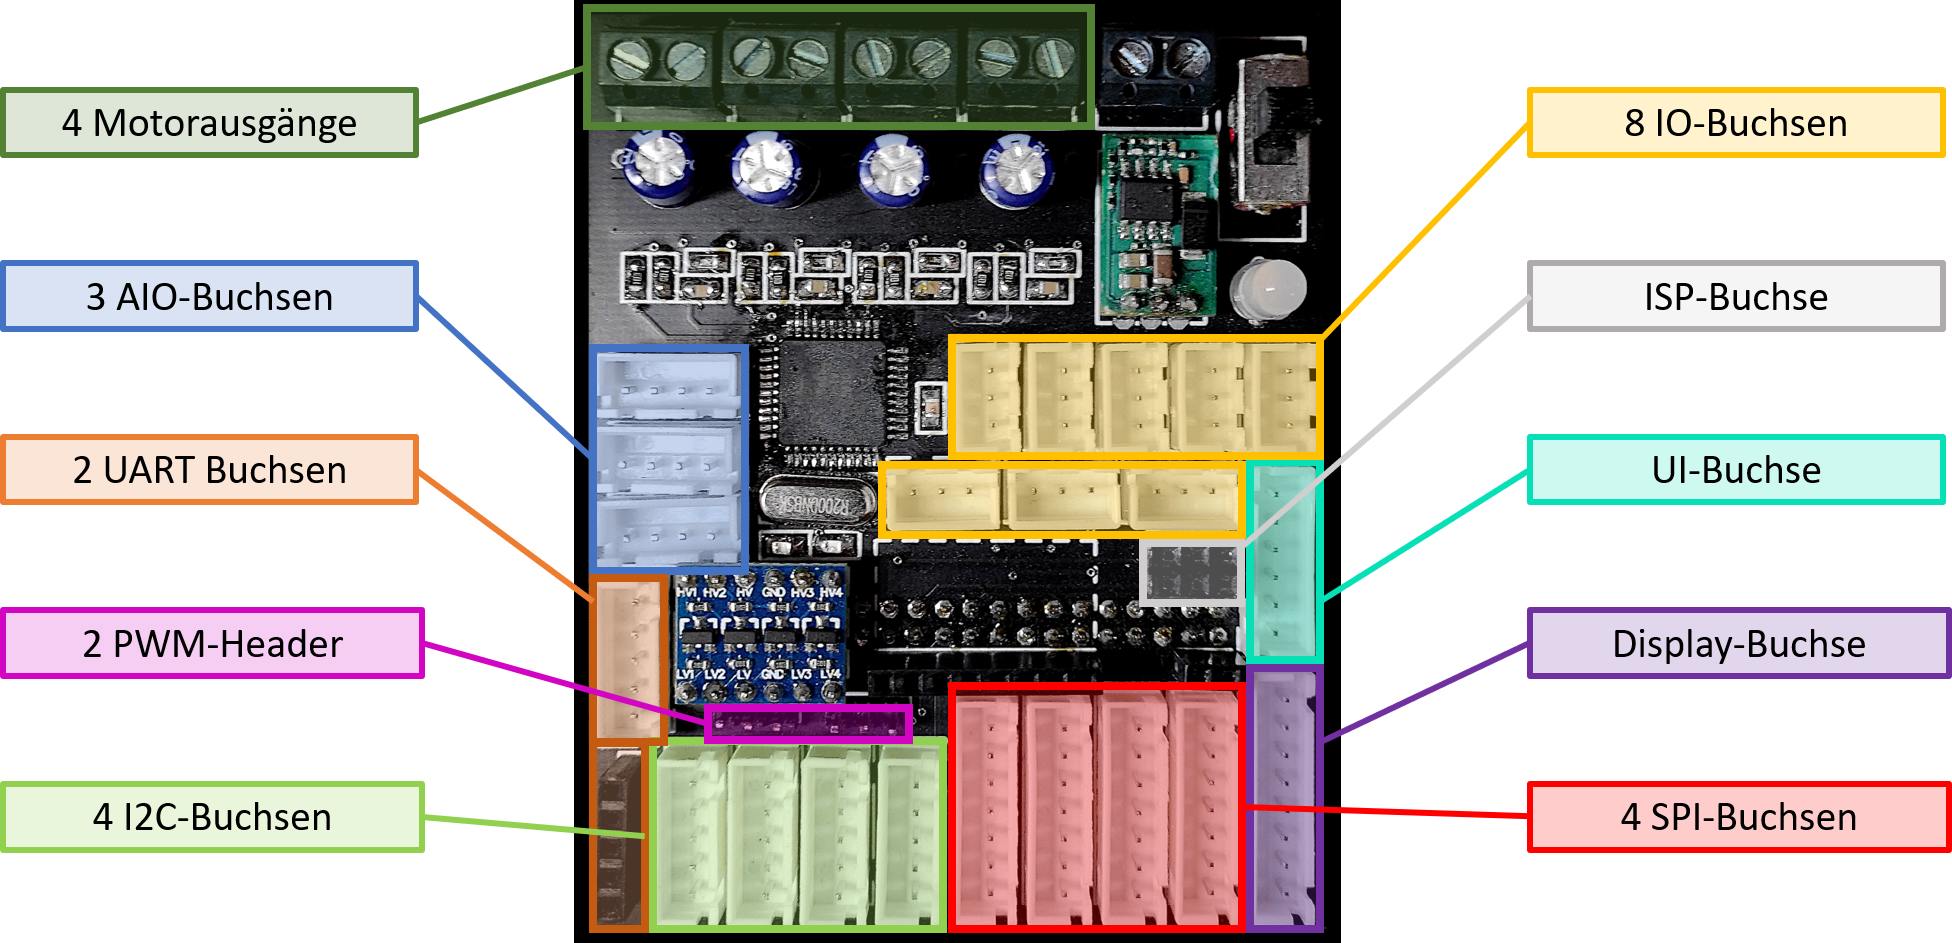
\includegraphics[width=\textwidth]{img/connectors.png}
\begin{center}\raisebox{6mm}{Abbildung 2: Stecker und Buchsen auf der Platine (Eigene Darstellung)}\end{center}
Für die Kommunikationen werden XH-Buchsen von J.S.T. Mfg. Co. verwendet, welche in ein 2.54mm-Rastermaß haben. Zusätzlich dazu werden für die ISP-Buchse, die beiden PWM-Header sowie der unteren UART-Buchse einfache 2.54mm Header beziehungsweise Buchsen verwendet, sodass dafür keine speziellen Kabel benötigt werden. Der Stromanschluss ist die Printklemme links vom Ein-Aus-Schalter, welcher sich im Eck rechts oben befindet. Die übrigen vier Printklemmen sind für die Motorausgänge.
\subsection{Komponenten}
Die wichtigste Hardware-Komponente ist ein Raspberry Pi Zero W, ein Single-Board-Computer basierend auf einem Broadcom BCM2835 SoC mit einer ARM11-Architektur. Das Raspberry Pi selbst hat eine Größe von 65 * 30mm und eine Höhe von circa 5mm. Es verfügt über einen Header mit 40 Pins, 26 dieser Pins sind so genannte GPIOs, die Kurzform für General Purpose Input Output.\\
Jeder dieser GPIOs ist direkt mit dem BCM2835 verbunden und erlaubt daher eine Maximalspannung von 3.3 V sowie einen maximalen Strom von 10 mA. Des weiteren sind noch acht Ground-Pins, zwei 3.3 V und zwei 5 V Pins vorhanden. Die Stromversorgung des Raspberry Pi erfolgt über die zwei 5 V Pins sowie einem Ground-Pin.
\\\\Als Subprozessor dient ein ATmega 644, ein 8-Bit Mikrocontroller von Atmel/Microchip, welcher in einem TQFP-44-Package verbaut ist. Diese SMD-Bauform ist quadratisch bei einer Seitenlänge von 12mm mit je elf Pins pro Seite. 32 dieser Pins sind GPIOs, welche mit einer Spannung von 5 V betrieben werden. Zusätzlich sind noch vier Ground-Pins, drei VCC-Pins, die zur Stromversorgung dienen, sowie ein AVCC- und AREF-Pin für den internen Analog-Digital-Wandler vorhanden. Die übrigen drei Pins sind der Reset-Pin, mit welchem der Chip deaktiviert werden kann, sowie zwei Pins, an die ein externer Quarz mit einer Frequenz von 20.0 MHz angeschlossen ist. \footnote{\fontfamily{phv}\selectfont vgl. Atmel Corporation, ATmega644/V, S. 2 und 362.}
\\\\Die Steuerung der Motor-Ausgänge erfolgt über vier Motortreiber vom Typ VNH7100ASTR von STMicroelectronics. Jeder Motortreiber enthält eine zweifache Halbbrücke, was eine Steuerung des Motors in beide Richtungen mit nur einem Motortreiber ermöglicht. Die Bauform dieser Komponente ist SO-16N, eine rechteckige Form mit einer Größe von 9.9 * 6.0 mm und je acht Pins auf den beiden längeren Seiten. Jeder Motortreiber kann einen Motor mit maximal 41 V bei 12 A steuern, die maximale Betriebsspannung beträgt 38 V. Die Drehrichtung sowie die Geschwindigkeit des Motors werden über dessen Input-Pins gesteuert. Diese sind mit dem ATmega verbunden. \footnote{\fontfamily{phv}\selectfont vgl. STMicroelectronics, VNH7100AS, S. 1 und 33.}
\\\\Auf der Platine ist auch ein Bosch BNO055 verbaut, ein Sensor, welcher ein Gyroskop, einen Magnetometer und einen Beschleunigungssensor in einem Bauteil kombiniert. Insgesamt kommt der BNO somit auf neun Freiheitsgrade. Der Sensor wird mit einer Spannung von 3.3 V versorgt, die Kommunikation mit dem Raspberry Pi findet über I2C statt. 
\subsection{Bussysteme}
Die Kommunikation zwischen den verschiedenen Komponenten erfolgt über folgende drei Protokolle:
\begin{compactitem}
    \item SPI
    \item I2C
    \item UART
\end{compactitem}\vspace{5mm}
Der ATmega 644 wird vom Raspberry Pi über SPI gesteuert, einem seriellen Bus mit vier Leitungen. Der Bus hat einen Master und beliebig viele Slaves, welche je mit einer so genannten Chip-Select-Leitung zum Master verbunden sind. Für die Datenübertragung hat der Bus eine Clock-Leitung, mit welcher der Master die Geschwindigkeit festlegt, sowie eine MOSI- und MISO-Leitung. MOSI bezeichnet hierbei den Output des Masters, daher kommt die Kurzform "MOSI" von "Master Output Slave Input". MISO ist die Leitung für den Datenverkehr vom Slave zu Master, die Kurzform steht für "Master Input Slave Output". Auf dem SPI-Bus werden die Daten synchron zur Clock-Leitung übertragen; es erfolgt immer ein Transfer eines Bytes in beide Richtungen gleichzeitig.
\\\\\\Der BNO055 ist über I2C mit dem Raspberry Pi verbunden, einem seriellen Bus mit zwei Leitungen. Der Bus hat eine Clock-Leitung, über welche der Master die Übertragungsgeschwindigkeit steuert, sowie eine Data-Leitung, auf welcher die Daten bidirektional übertragen werden. Das erste Byte jeder Übertragung besteht aus der Adresse des Slaves, an den sich die Kommunikation richtet, sowie einem Bit, welches die Richtung festlegt. Daher sind auf einem Bus maximal 127 Slaves und ein Master möglich. Die beiden Leitungen sind mit Pull-Up Widerständen versehen und werden zu Ground durchgeschalten, um eine logische Null am Bus zu senden.
\\\\\\Für eine einfache Datenübertragung zwischen dem Raspberry Pi und einem Computer steht auch noch UART zur Verfügung. UART ist ein asynchroner Bus mit je einer Datenleitung pro Richtung. Der Bus selbst unterstützt jedoch nur zwei Geräte, die je ein Empfänger- und einen Transmittermodul besitzen. Die Geschwindigkeit der Datenübertragung, Baudrate genannt, muss für beide Geräte ident sein, damit die Daten korrekt empfangen werden können. Auf dieser Platine wird eine Baudrate von 115200 Bit/s genutzt, da die meisten UART-Komponenten diese Baudrate verwenden. Der optionale Anschluss eines UART-to-USB-Wandlers erfolgt über die untere UART-Buchse auf der Platine.
\subsection{Pinouts}
Bei der Spannungsversorgung muss die positive Leitung auf der Seite des Ein-Aus-Schalters angeschlossen werden, damit die Komponenten richtig mit Strom versorgt werden.\\
Um einen STromfluss in die falsche Richtung zu verhindern, ist eine Diode vom Typ ES3D von On Semiconductors verbaut. Die Diode ist für maximal 200 V und einen Spitzendurchlassstrom von 100 A ausgelegt. Wenn bei den Motorterminals die Kabel vertauscht werden, ändert dies lediglich die Drehrichtung des Motors.\\\\
Jede der XH-Buchsen verhindert ein verpoltes Anstecken eines Gegensteckers. Alle Buchsen besitzen einen Ground-Pin und einen 5V-Pin, zusätzlich ist bei allen außer den IO-Buchsen auch ein 3.3V-Pin vorhanden. 
\begin{compactitem}
    \item Die IO-Buchsen haben drei Pins: GND, +5V und IO. IO steht hier für den Pin des ATmegas, welcher als Input sowie auch als Output verwendet werden kann.
    \item Die ADC-Buchsen haben vier Pins: GND, +3.3V, +5V und AIO. AIO bezeichnet den Pin, der als Input, Output und analoger Input genutzt werden kann.
    \item Die UART-Buchse hat fünf Pins: GND, +3.3V, +5V, RX und TX. RX ist die Reciever-Leitung des Raspberry Pi, TX die Transmitter-Leitung.
    \item Die I2C-Buchsen haben ebenfalls fünf Pins: GND, +3.3V, +5V, SCL und SDA. SCL und SDA werden mit 5V betrieben.
    \item Die User Interface-Buchse hat sechs Pins: GND, +5V und vier GPIOs. Jeder GPIO wird mit einer Maximalspannung von 3.3V betrieben und ist nicht 5V-kompatibel.
    \item Die SPI-Buchsen haben sieben Pins: GND, +3.3V, +5V, MOSI, MISO, SCL und CS. Alle angeschlossenen Geräte dürfen nur als SPI Slave arbeiten und MISO mit maximal 5V steuern. Chip Select hat eine Spannung von 3.3V.
    \item Die Display-Buchse hat acht Pins: GND, +3.3V, +5V, SCL, MISO, MOSI, CS und DC. Die Buchse ist eine SPI-Buchse mit einem weiteren Pin, dem Data-Command-Pin, welcher bei den meisten Displays benötigt wird.
\end{compactitem}
Der ISP-Stecker entspricht dem In System Programmer mkII-Standard von Atmel/Microchip, welcher ein SPI-Interface ohne Chip Select, ein Ground-Pin, ein VCC-Pin sowie ein Reset-Pin beinhaltet. Die PWM-Header entsprechen den normalen Servo-Anschlüssen mit einem 5V-Pin, einem Ground- und einem PWM-Pin. Der PWM-Pin hat jedoch eine maximale Spannung von 3.3V, da das PWM-Signal über das Raspberry PI erzeugt wird. Der UART-Header ist für einen UART/TTY to USB-Wandler angepasst, der Pinout lautet: +3.3V, RX, TX, GND, +5V.
\subsection{SMD-Größen}
Alle passiven Komponenten mit nur zwei Anschlüssen außer dem Quarz sowie den Kondensatoren für die Motortreiber sind als SMD-Komponenten verbaut. SMD ist die Kurzform von "Surface Mounted Device", somit sind dies Bauteile, welche nur auf einer Seite der Platine montiert und verlötet werden. Das Gegenteil hierzu sind Through-Hole-Komponenten, welche Pins besitzen, die durch ein Lötauge gesteckt werden und auf der anderen Seite verlötet werden. Alle diese passiven Komponenten sind in einem 0805-Formfaktor verbaut.\\\\
0805 steht hierbei für die Größe des einzelnen Bauteils in $\frac{1}{100}$ Zoll. Die erste Zahl definiert die Länge, die zweite die Breite. Die Höhe der Komponenten wird nicht über den Formfaktor angegeben, ist jedoch meist kleiner oder gleich der Breite. Somit ergibt sich für die Komponenten eine Größe von 2.032 * 1.27mm bei einer maximalen Höhe von 1.27mm. Die Entscheidung fiel auf diese Bauform, da jene noch händisch lötbar ist jedoch gleichzeitig wenig Platz auf der Platine einnimmt. 
\\\\Nur die Diode beim Stromanschluss hat eine größere Bauform, da diese bei Spannungen von 35 V Spitzenströme über 10 A aushalten muss. Hierfür wird ein SMC / DO-214AB -Formfaktor genutzt, welcher eine Länge von 8 mm, eine Breite von 6 mm sowie eine Höhe von 2.65mm hat.\footnote{\fontfamily{phv}\selectfont vgl. Fairchild, ES3A-ES3J Fast Rectifiers, S. 4.}
\subsection{Abgrenzung der Spannungsniveaus}
Die Platine wird über eine Printklemme mit Strom versorgt, die Inputspannung muss hierbei zwischen 7V und 35V liegen. Das Raspberry Pi und der ATmega644 benötigen eine Versorgungsspannung von 5V, daher ist ein OKI-78SR-Spannungswandler von Murata Power Solutions verbaut, welcher eine Outputspannung von 5V mit 1.5A erzeugt. Die Motortreiber werden mit der vollen Batteriespannung versorgt.
\begin{wrapfigure}[11]{r}{0.4\textwidth}
\vspace*{-6mm}{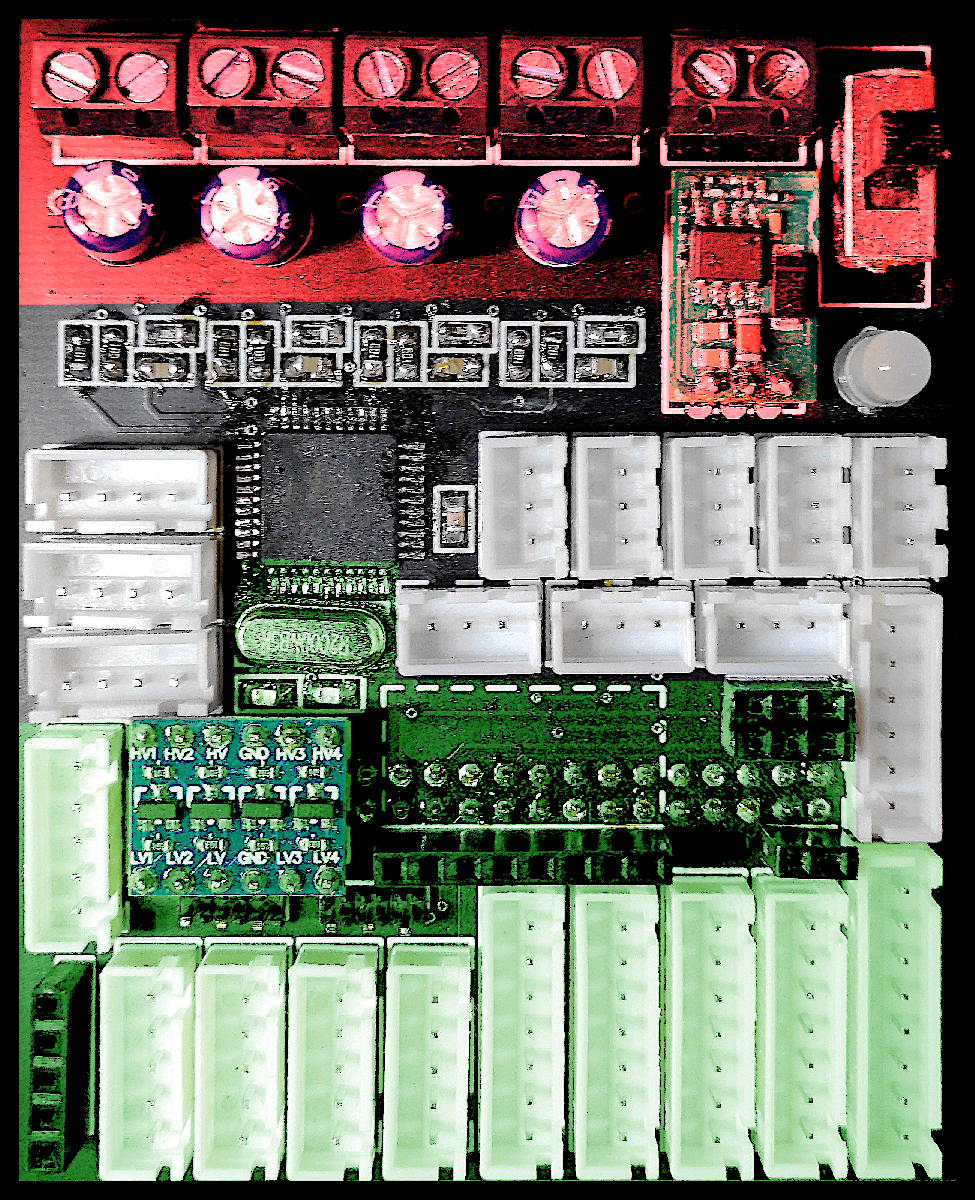
\includegraphics[width=0.4\textwidth]{img/levels.png}}\\
\raisebox{4mm}{Abbildung 3: Grafische Darstellung}\\
\raisebox{5mm}{der Spannungsniveaus auf der}\\
\raisebox{6mm}{Platine (Eigene Darstellung)}
\end{wrapfigure}
Eine Abgrenzung des VCC-Bereiches und des 5V-Bereiches ist wichtig, da die Motortreiber kurzzeitig Stromspitzen von über 10 A erzeugen können. Diese können bei benachbarten Leitungen Spannungsdifferenzen hervorrufen, welche die Maximalspannung mancher Bauteile überschreitet. Diese Spannungsspitzen können ebenfalls Kommunikationen stören, indem die Spannung eines logischen LOW über die Mindestspannung für ein logisches HIGH steigt und somit als logisches HIGH vom Empfänger der Kommunikation erkannt wird.\\
Die Abbildung 3 stellt in rot den gesamten Bereich dar, der mit voller Batteriespannung betrieben wird und durch Stromspitzen der Motortreiber beeinflusst wird. Die Leitungen für die Versorgungsspannung und Ground haben eine Breite von 4.5mm, sodass jene hohe Ströme bei geringer Erwärmung durch den Innenwiderstand leiten können.
\\\\In grün ist der Bereich mit Kommunikationen markiert, welcher durch den Spannungswandler mit einer stabilen Spannung von 5V versorgt wird. Nur in dem Moment, wo das Board eingeschalten wird, gibt es eine kurze Stromspitze auf dieser Seite, jedoch sind zu diesem Zeitpunkt noch keine Komponenten aktiv. Dadurch, dass eine räumliche Trennung von 15mm zwischen den beiden Bereichen liegt, können keine 
Spannungsspitzen durch Induktion im grünen Bereich entstehen.
\subsection{Kondensatoren und Schwingquarz}
Jeder der vier Motortreiber hat zwischen den VCC- und Ground-Pins einen Elektrolytkondensator mit einer Kapazität von 270$\mu$F. Das Datenblatt der VNH7100ASTR-Motortreiber sieht diese Kondensatoren zwischen VCC und Ground vor, sie können zusätzlich noch durch je einen 100 nF-Kondensator ergänzt werden, welcher jedoch nur zum Ausgleich hochfrequenter Schwingungen dient. Die großen Kondensatoren unterstützen beim Ausgleich von Spannungseinbrüchen über einen kurzen Zeitraum, sodass die Geschwindigkeit des Motors dennoch konstant bleibt. 
\\\\Neben dem ATmega644 ist ein kleiner Kondensator mit einer Kapazität von 100 nF zwischen der +5V-Leitung und der Ground-Leitung verbaut, welcher Schwingungen auf der Spannungsversorgung eliminiert.\\
Bei dem ATmega ist dies für akkurate Messwerte durch den Analog-Digital-Wandler wichtig, ebenso für den Schwingquarz, damit der Takt stabil bleibt. Eine instabile Taktrate des ATmega kann zu Problemen bei Verzögerungen führen, da diese in eine fixe Anzahl an Warte-Anweisungen kompiliert werden. Ebenfalls könnten bei einer variierenden Taktrate Probleme bei diversen Kommunikationen wie UART entstehen. Auf dieser Platine wird der ATmega über SPI gesteuert, da SPI ein synchroner Bus ist.
\\\\Das Raspberry PI sowie der BNO055 benötigen keinen externen Kondensator zur Spannungsstabilisierung, da beide Komponenten einen bereits auf dem jeweiligen Board haben. Der BNO055 ist auf einem Breakout-Board verbaut, welches einen Schwingquarz mit 32.768 MHz sowie die dazugehörigen Bauteile zur Spannungsstabilisierung beinhaltet.
\\\\Die Taktrate des ATmega644 wird durch einen externen Schwingquarz gesteuert, welcher eine Frequenz von 20 MHz hat, was in der vollen Leistung des ATmegas resultiert. Der Schwingquarz hat zwei Pins, welche direkt mit den XTAL1- und XTAL2-Pins des ATmega verbunden sind. Zusätzlich ist jeder Pin des Schwingquarzes über einen 22 pF-Kondensator mit Ground verbunden. Die Kapazität der Kondensatoren wird über die Eigenkapazität des Schwingquarzes sowie der Kapazität der Leitungen in der dazugehörigen Schaltung berechnet.
\subsection{Levelshifting}
Alle GPIOs des Raspberry PI haben eine Maximalspannung von 3.3V, jedoch nutzen viele Komponenten eine Kommunikationsspannung von 5V.\\
Um eine Kommunikation zwischen einer 3.3V-Komponente und einer 5V-Komponente zu ermöglichen, kommt das so genannte Levelshiftig zum Einsatz. Auf der Platine werden folgende zwei Levelshifting-Methoden verwendet:
\vspace{2mm}
\begin{compactitem}
    \item Spannungsteiler um 5V auf 3.3V zu reduzieren
    \item Bidirektionale Levelshifter mit Mosfets
\end{compactitem}
\vspace{6mm}
Bei den meisten GPIOs des Raspberry Pi, welche als Output genutzt werden, genügen die 3.3V, da die meisten 5V-Komponenten ab 2.5V ein logisches HIGH erkennen. Die einzigen Ausnahmen sind I2C und UART, für welche die Spannung auf 5V erhöht werden muss. Auf der Platine ist ein bidirektionaler Levelshifter mit 4 Kanälen verbaut, welcher für die I2C-Leitungen SDA und SCL sowie für die UART Recieve- und Transmitleitungen verwendet wird. Bei jedem Kanal ist ein Mosfet verbaut, welcher den Kanal durchschaltet. Des weiteren ist auf der 3.3V-Seite jedes Kanals ein 10 k$\Omega$ Pull-Up Widerstand verbaut, der die Spannung auf +3.3V zieht. Auch auf der 5V-Seite ist ein 10 k$\Omega$ Pull-Up Widerstand angebracht, welcher die Leitung auf +5V zieht. Wenn der Kanal auf der 3.3V-Seite nun auf Ground durchgeschalten wird, dann existiert eine positive Spannung zwischen Gate und Source des Mosfets, somit schaltet dieser durch und die 5V-Seite wird auch mit Ground verbunden, wodurch ein logisches LOW entsteht. Um eine Signalübertragung in die umgekehrte Richtung zu ermöglichen, hat der Mosfet eine Diode verbaut, welche einen Stromfluss von der 3.3V-Seite zur 5V-Seite erlaubt. Sobald auf der 5V-Seite nun zu Ground durchgeschalten wird, fällt die Spannung auch auf der 3.3V-Seite auf ein logisches LOW.
\\\\\\Um ein 5V-Signal auf 3.3V zu reduzieren, kommt ein einfacher Spannungsteiler mit zwei Widerständen zum Einsatz, dies wird zum Beispiel bei der MISO-Leitung des SPI-Busses benötigt, da die Slaves diese mit maximal 5V steuern, das Raspberry Pi aber nur 3.3V verträgt. Das Verhältnis der Widerstände muss dem Verhältnis der Spannungen entsprechen, bei 5V zu 3.3V beträgt dieses 1.5152 : 1. Da zwischen 5V und Ground optimalerweise ein Mindestwiderstand von 5 k$\Omega$ existieren sollte, lauten die Widerstände zur Spannungsteilung 2.4 k$\Omega$ und 4.7 k$\Omega$, dies entspricht einem Verhältnis von 1.51 : 1 bei Berechnung des Gesamtwiderstands relativ zu dem 4.7 k$\Omega$-Widerstand. Der Gesamtwiderstand zwischen dem 5V-Signal und Ground beträgt somit 7.1 k$\Omega$, somit wird der Strom auf 0.7 mA begrenzt. Der Aufbau dieses Spannungsteilers sieht folgendermaßen aus: die 5V-Signalleitung ist über einen 2.4 k$\Omega$-Widerstand mit der 3.3V-Signalleitung verbunden, von dieser führt ein 4.7 k$\Omega$-Widerstand zu Ground. 
\newpage\section{Bootloader}
In dieses Kapitel wird der Bootvorgang des Raspberry Pis sowie die Toolchain, welche zur Kompilierung verwendet wird, beschrieben. Ebenfalls wird der Code des eigenen Bootloaders erklärt.
\subsection{Bootprozess des Raspberry Pi}
Der Broadcom BCM2835-SoC, welcher auf dem Raspberry Pi Zero W verbaut ist, besteht aus einem ARM1176JZF-S-CPU, einem Single-Core Prozessor mit einer Taktrate von 1 GHz, sowie einem Broadcom Videocore IV mit einer Taktrate von 250 MHz. Das Raspberry Pi Zero W kann über die SD-Karte und über USB booten, in dieser Arbeit wird jedoch nur der Boot über eine SD-Karte genutzt. Die Bootreihenfolge sieht folgendermaßen aus:
\begin{center}
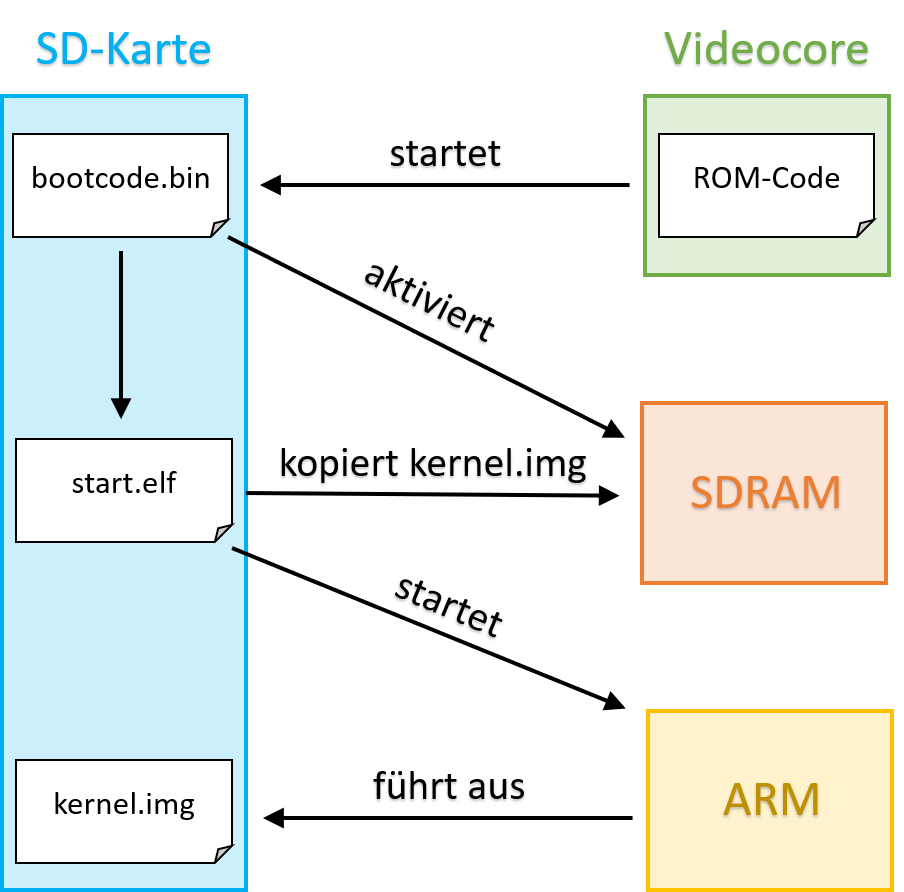
\includegraphics[width=0.6\textwidth]{img/bootloader.png}
\end{center}
\begin{center}
Abbildung 4: Bootprozess des Raspberry Pi (Eigene Darstellung)
\end{center}
Zu Beginn bleibt der ARM noch ausgeschaltet, der Videocore führt Code vom ROM aus, welcher die SD-Karte einliest und den zweiten Teil des Bootloaders, \textit{bootcode.bin}, lädt und ausführt. \textit{bootcode.bin} aktiviert den SDRAM und lädt die GPU-Firmware \textit{start.elf}, welche das kompilierte Programm in den SDRAM lädt. Zum Abschluss wird der ARM gestartet und die Anweisungen des Programms ab der SDRAM-Adresse 0x8000 ausgeführt.\footnote{\fontfamily{phv}\selectfont vgl. Soininen, Jonne: Linux boot loader and boot in Raspberry Pi, S. 4.}
\\\\\textit{bootcode.bin} und \textit{start.elf} sind Dateien der Raspberry Pi Foundation, welche auf Github.com in der Repository "firmware" des Nutzers "raspberrypi" im Ordner "boot" gefunden werden können. Um eine SD-Karte als Bootmedium einzurichten, muss diese mit dem Filesystem FAT32 ausgestattet sein und die beiden Dateien sowie das kompilierte Programm, \textit{kernel.img}, beinhalten.
\subsection{Toolchain}
Für die Kompilierung des Codes kommt die arm-none-eabi-Toolchain der GNU Compiler Collection zum Einsatz. Diese Toolchain ist für die Programmiersprachen C, C++ und Assembly auf ARM-Bare-Metal-Plattformen geeignet. Eine Bare-Metal-Plattform ist eine Plattform, auf welcher kein Betriebssystem oder ähnliche Software läuft, das den Arbeitsspeicher oder diverse Schnittstellen verwaltet. Der Vorteil einer Bare-Metal-Plattform ist, dass bei höchster Performance nur das Wichtigste ausgeführt wird. Würde auf dem Raspberry Pi zum Beispiel ein Linux laufen, dann würde ein Filesystem sowie das Terminal im Hintergrund geladen werden und somit die allgemeine Performance verschlechtern.
\\Zum Kompilieren eines C/C++/Assembly-Programmes, wird der Konsolenbefehl \textit{arm-none-eabi-g++} verwendet, da dieser .c / .cpp / .s-Dateien direkt in eine .elf-Datei kompiliert. Dieser Befehl kombiniert den C/C++ Preprocessor, den Compiler, den Assembler sowie den Linker, daher kann mit einem Befehl ein ausführbares Programm erstellt werden. Da der Befehl so viele Kompilierungsschritte umfasst, gibt es auch viele Argumente, folgende werden für die Kompilierung verwendet:\\\\
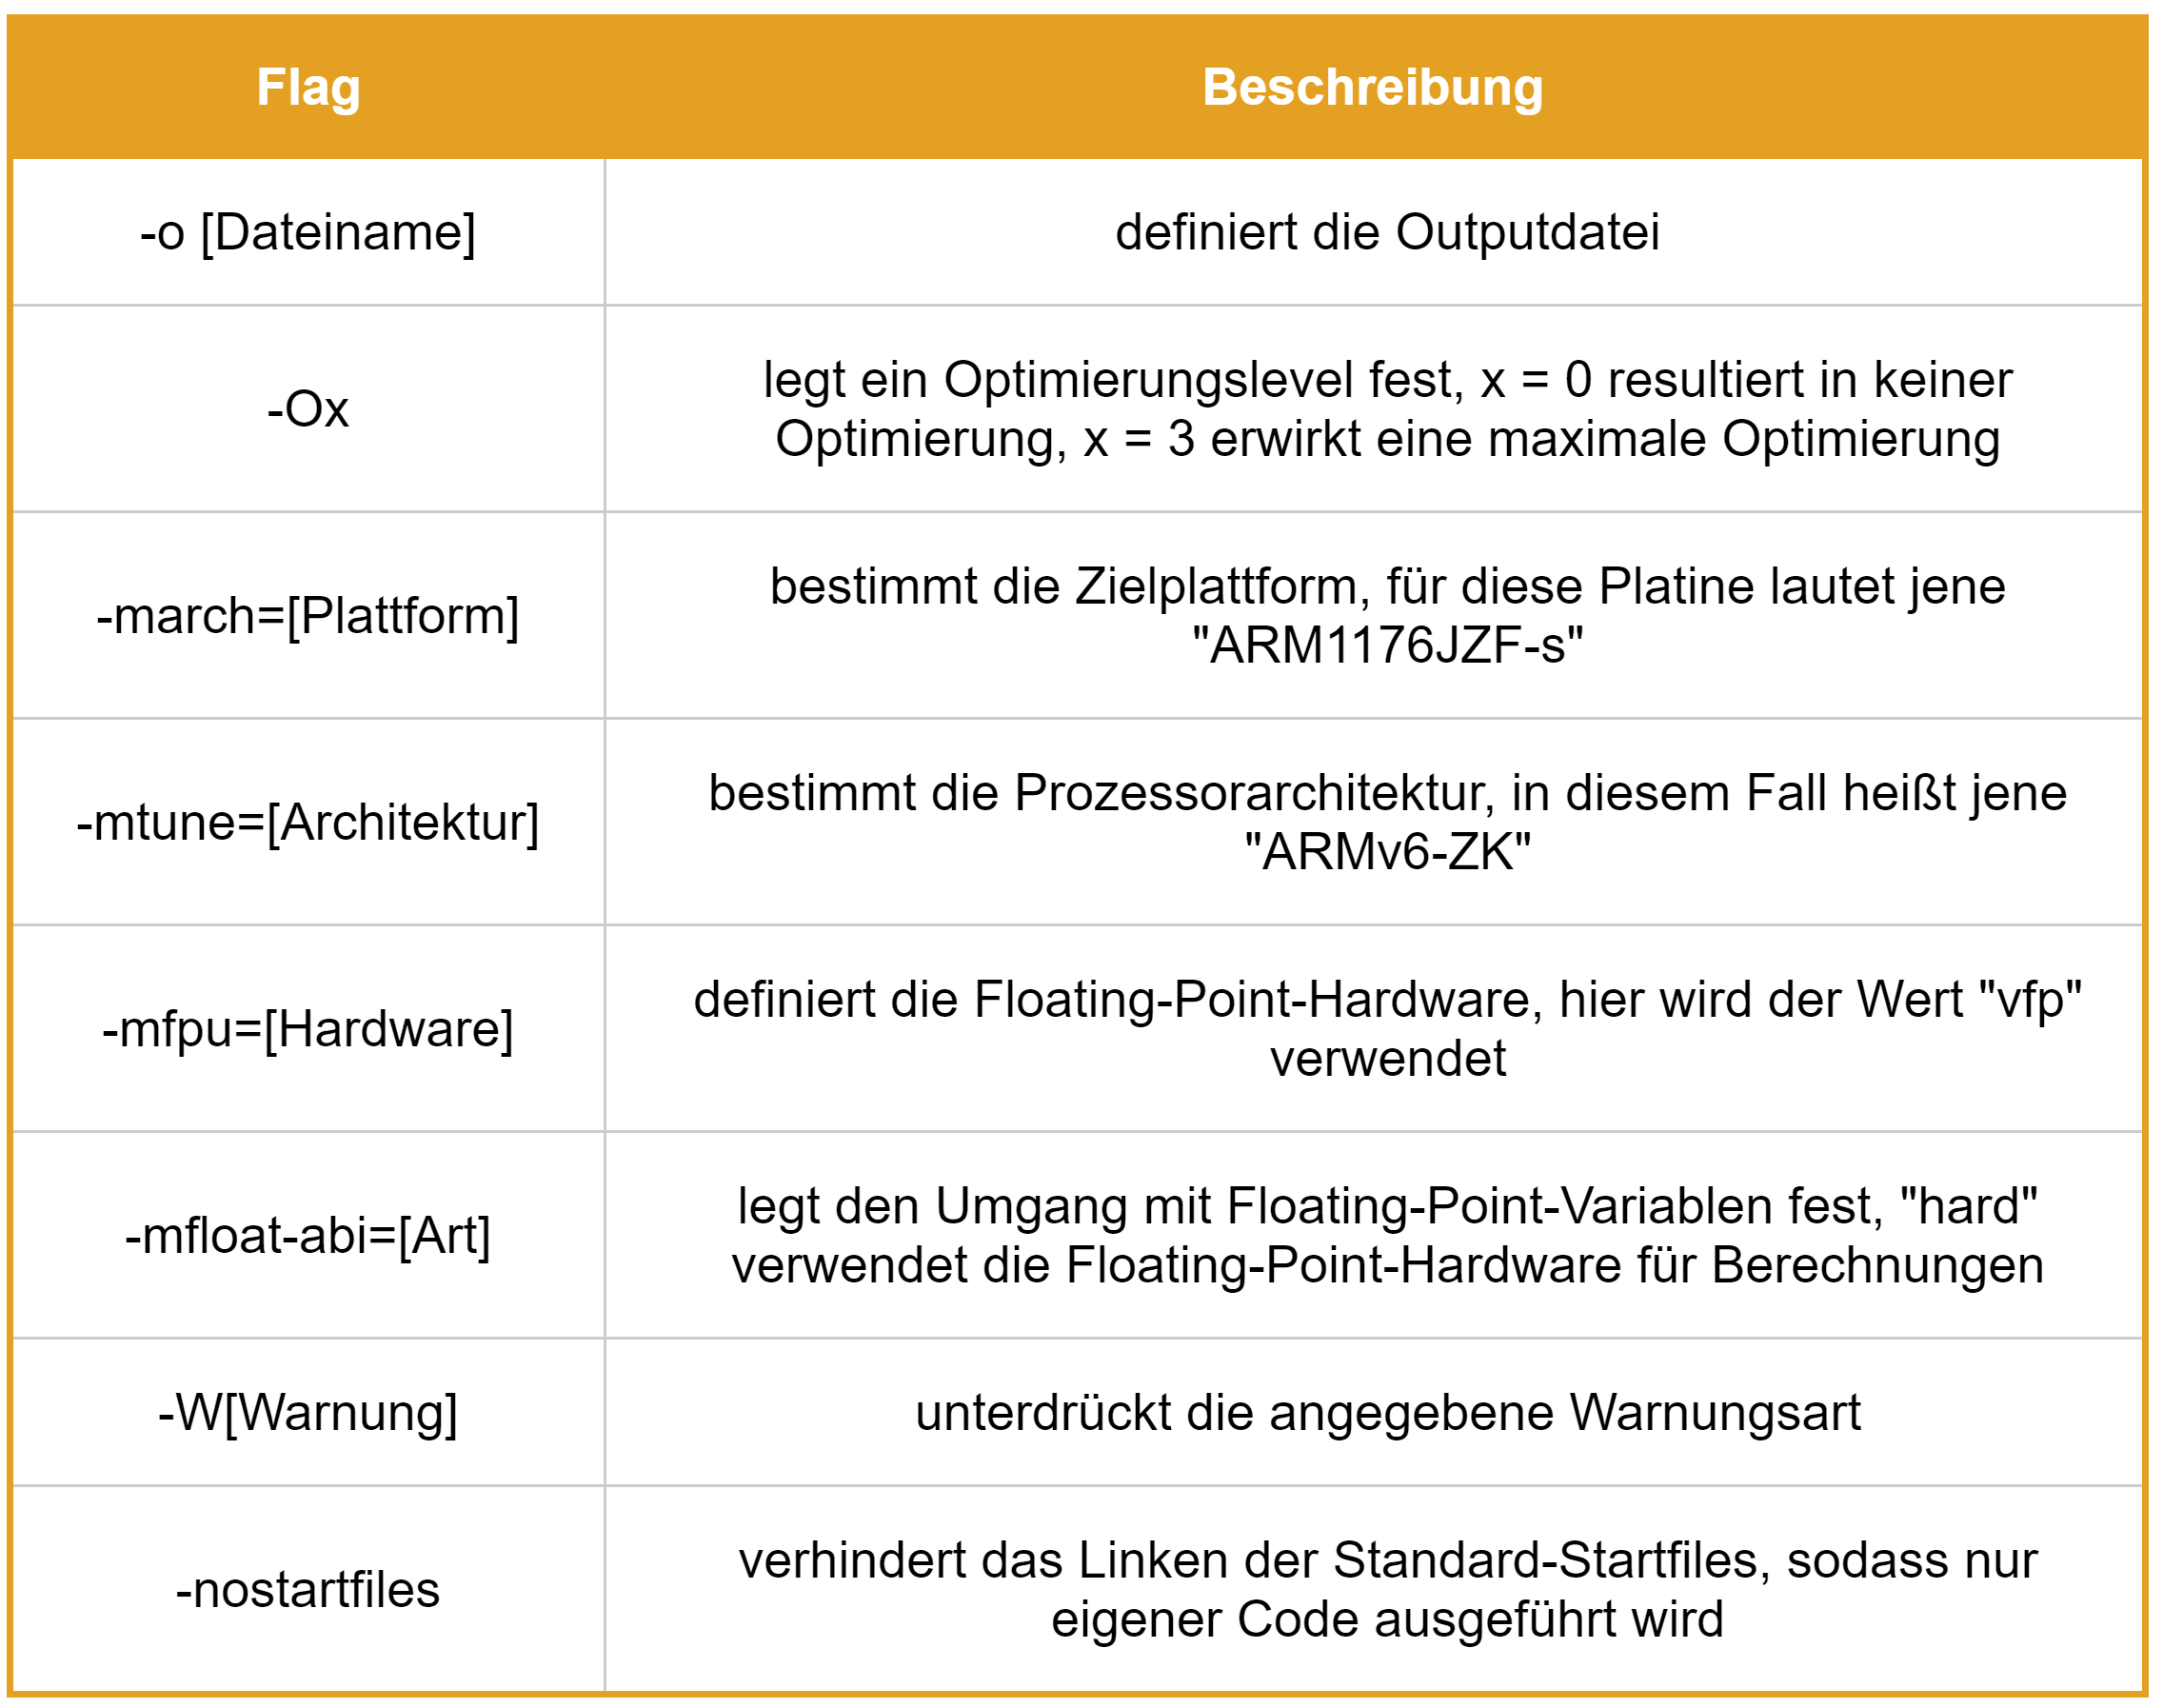
\includegraphics[width=\textwidth]{img/flags.PNG}
\begin{center}
\vspace{-5mm}
Abbildung 5: Tabelle der verwendeten Compiler-Argumente (Eigene Darstellung)
\end{center}
Die zu kompilierenden Dateien werden ohne einen Präfix und durch Leerzeichen getrennt übergeben. Für Assembly-Dateien werden der Preprocessor und der Kompilierungsschritt übersprungen.\\
Um aus der Ouput-Datei nun ein Datenträgerimage (.img) zu erzeugen, wird der Befehl \textit{arm-none-eabi-objcopy} mit dem \textit{-binary} Argument verwendet. Für die Kompilierung des Source-Codes werden folgende zwei Befehle nacheinander ausgeführt:\\
\begin{compactitem}
    \vspace{-5mm}
    \item arm-none-eabi-g++ -Wwrite-strings -nostartfiles -mfloat-abi=hard -O0 -mfpu=vfp\\
     -march=armv6zk -mtune=arm1176jzf-s -o kernel.elf [Dateien]
    \vspace{2mm}
    \item arm-none-eabi-objcopy kernel.elf -O binary kernel.img
\end{compactitem}
\subsection{Bootloader in Assembler}
Die Aufgabe des Bootloaders besteht darin, den Vector-Floating-Point-Coprozessor (VFP) des ARM zu aktivieren, sowie den Stack Pointer auf die Adresse 0x8000 zu setzen und anschließend die Funktion \textit{main} des C++-Programmes aufzurufen. \\
\begin{minted}{gas}
.globl _start
_start:
\end{minted}
Als Erstes wird die globale Funktion \textit{\_start} definiert, welche der Startpunkt des Programmes ist. Der Compiler sucht nach der \textit{\_start}-Funktion, wenn diese jedoch nicht gefunden wird, startet das Programm bei der Funktion \textit{main}.\\
\begin{minted}{gas}
    mrc p15, 0, r0, c1, c0, 2
    orr r0,r0,#0x300000
    orr r0,r0,#0xC00000
    mcr p15, 0, r0, c1, c0, 2
\end{minted}
\vspace{-2mm}
Mit der MRC-Anweisung wird das c1-Register ausgelesen und in das Register r0 kopiert. Nun werden in r0 die Bits 20-23 auf 1 gesetzt und das Ergebnis mit der MCR-Anweisung wieder in das Register c1 geschrieben.\\
\begin{minted}{gas}
    mov r0,#0x40000000
    fmxr fpexc,r0
    mov sp,#0x00008000
    bl main
\end{minted}
\vspace{-2mm}
Anschließend wird das Register r0 mit dem Hexadezimalwert 0x40000000 beschrieben und mit der Anweisung FMXR in das FPEXC-Register geschrieben, um die VFP-Unit zu aktivieren. Danach wird der Stack Pointer auf die Adresse 0x8000 verschoben, wo die erste Anweisung des C++-Programms liegt. Zuletzt wird mit der Branch-Link-Anweisung (BL) die Funktion \textit{main} aufgerufen.
\newpage\section{Raspberry Pi Software}
Dieses Kapitel beinhaltet alle Teile des Source-Codes der Library, welche eine einfache Steuerung aller Hardware-Controller des Raspberry Pis erlaubt.
\subsection{Grundinformationen}
Die C++-Library besteht ausschließlich aus Header-Dateien, welche mit \textit{\#include} in Source-Dateien eingebunden werden können. Dies hat den Vorteil, dass nicht jede einzelne Datei im Vorhinein in eine Object-Datei kompiliert werden muss, welche dann gemeinsam in eine Shared-Object-Datei zusammengefügt werden würden. Eine Shared-Object-Datei ist eine Binärdatei, somit wären Änderungen im Source-Code der Library nicht mehr möglich.
\\\\Jede Header-Datei enthält den \textit{\#pragma once} Include-Guard, welcher eine mehrfache Definition der gleichen Klassen und Funktionen verhindert. Die Datei \textit{VWAPI.hpp} inkludiert alle anderen Header-Dateien, somit genügt \textit{\#include "VWAPI.hpp"} um Zugriff auf alle Funktionen der Library zu erhalten. Zu Beginn eines jeden Programmes sollte die Funktion \textit{init }der Klasse \textit{VWAPI} aufgerufen werden, welche alle GPIOs richtig konfiguriert und die Verbindung mit dem ATmega überprüft. Zum Aufrufen dieser Funktion genügt die Anweisung \textit{VWAPI().init();}.
\\\\Der ARM11-Prozessor des BCM2835-SoC ist ein 32-Bit Prozessor, somit können die Speicheraddressen 0x00000000 bis 0xFFFFFFFF adressiert werden. Alle GPIOs werden über den Videocore gesteuert, daher sind die Adressen im Datenblatt des BCM2835 als Videocore-Adressen angegeben. Wenn nun von dem Programm, das auf dem ARM läuft, ein IO-Register adressiert wird, muss auf das Memory-Mapping geachtet werden. Alle IO-Adressen sind bei dem Videocore ab der Adresse 0x7F000000 zu finden, diese sind für dem ARM ab der Adresse 0x20000000 erreichbar.
\\\\Register können direkt mit Werten beschrieben werden, jedoch können auch OR, XOR und AND-Operationen auf diese angewendet werden. Wichtig ist hierbei, dass jene bei Registern mit Write-only Bits fehlschlagen und keine Auswirkung haben. Das Beschreiben eines Read-only Bits hat keine Wirkung, jedoch schlägt nicht der gesamte Schreibvorgang fehl. Alle Register werden im Code über volatile unsigned int*-Pointer adressiert. Der Typ unsigned Integer erlaubt hierbei die Nutzung aller 32 Bits des Registers, ohne dass negative Werte Auswirkungen auf das gesamte Register haben. Die Eigenschaft volatile bestimmt, dass der Wert der Variable sich außerhalb des Programmes ändern kann, daher wird immer der aktuellste Wert von der Speicheradresse abgerufen.
\subsection{GPIO}
Die Steuerung der GPIOs erfolgt über die Register mit der Grundadresse 0x20200000. Da der BCM2835 54 GPIOs hat, sind alle Funktionen auf mehrere Register aufgeteilt, weil pro Register nur 32 Bit zur Verfügung stehen. Alle Funktionen der GPIOs werden mit Hilfe der Klasse \textit{GPIO} gesteuert. Die Register sind folgendermaßen angeordnet:\\\\
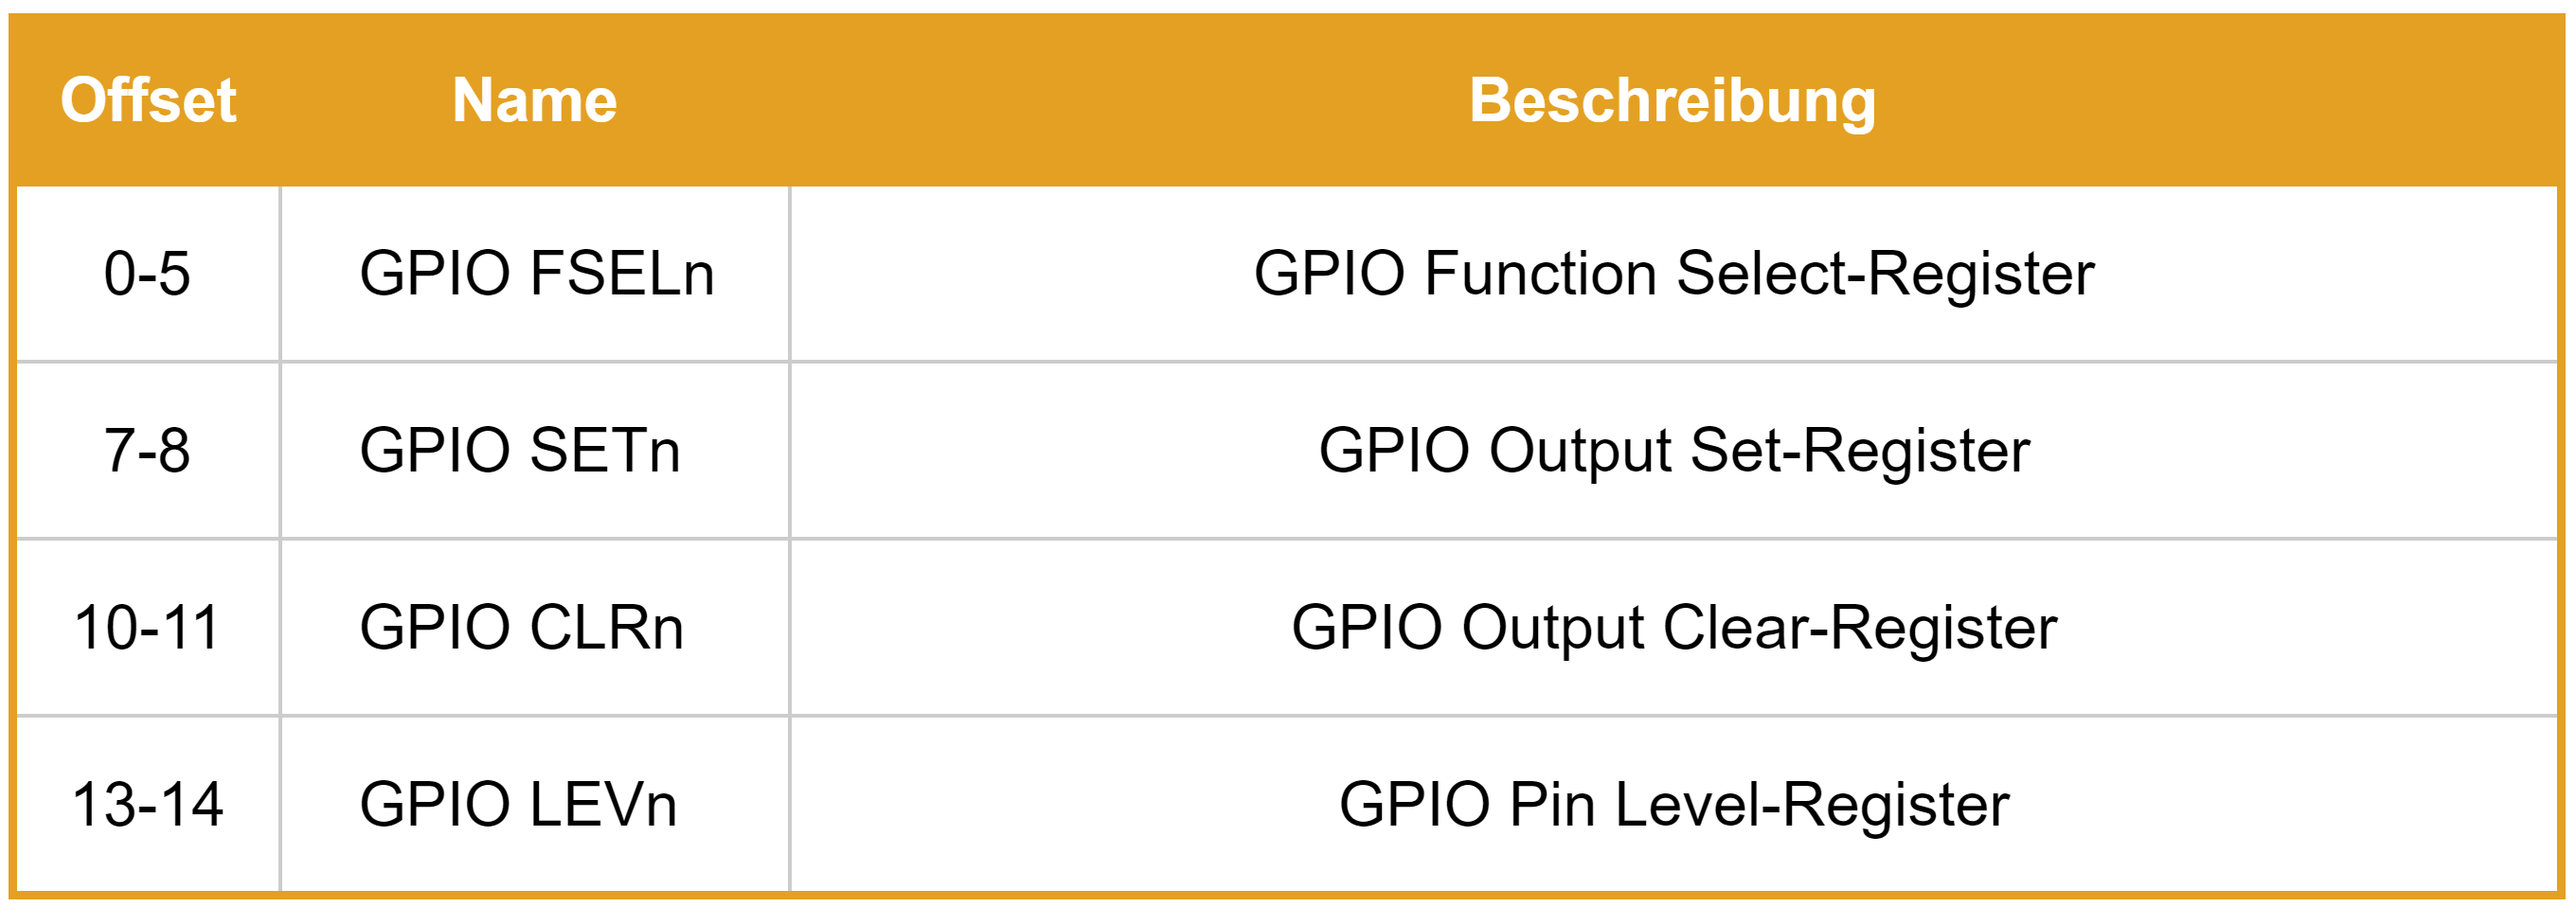
\includegraphics[width=\textwidth]{img/gpio_table.png}
\begin{center}\raisebox{9mm}{Abbildung 6: Register des GPIO-Controllers (Eigene Darstellung)}\end{center}
\begin{minted}{c++}
class GPIO {
    volatile unsigned int* reg;
    char id;
public:
    enum Mode { INPUT, OUTPUT, ALT0 = 4, ALT1 = 5, 
                ALT2 = 6, ALT3 = 7, ALT4 = 3, ALT5 = 2};
\end{minted}
\vspace{-2mm}
Die Klasse \textit{GPIO} enthält einen volatile unsigned int*-Pointer sowie eine char, welche die ID des Pins speichert. Des weiteren definiert die Klasse das Enum \textit{Mode}, welches alle Modi der GPIOs enthält und diese mit der internen ID versieht.\\
\begin{minted}{c++}
    GPIO() {}
\end{minted}
\begin{minted}{c++}
    GPIO(char pin) {
        reg = (unsigned int*) 0x20200000;
        id = pin;
    }
\end{minted}
\begin{minted}{c++}
    GPIO(char pin, Mode mode) {
        reg = (unsigned int*) 0x20200000;
        id = pin;
        setMode(mode);
    }
\end{minted}
\vspace{-2mm}
Es gibt 3 Konstruktor, mit denen eine Instanz der Klasse erstellt werden kann. Der Default-Konstruktor hat keine Wirkung und dient nur zur Erstellung leerer Instanzen. Wenn nur ein Pin übergeben wird, wird dieser in die Variable \textit{id} kopiert. Sollte auch noch ein Mode übergeben werden, wird die Funktion \textit{setMode(mode)} aufgerufen. Beide Konstruktor setzen die Adresse des Pointers auf 0x20200000, der Grundadresse aller GPIO-Register.\\
\begin{minted}{c++}
    Mode getMode() {
        return static_cast<Mode>(
            (reg[id/10] >> ((id % 10) * 3)) & 0x07);
    }
\end{minted}
\begin{minted}{c++}
    void setMode(Mode mode) {
        reg[id/10] &= ~(0x07 << ((id % 10) * 3));
        reg[id/10] = ((mode & 0x07) << ((id % 10) * 3));
    }
\end{minted}
\vspace{-2mm}
Der Modus eines Pins wird in den GPIO Function Select-Registern gespeichert, GPIO Function Select 1 ist beispielsweise für die Pins 10 - 19 zuständig. Jeder Pin hat 3 Bits im dazugehörigen Register, welche den Modus darstellen. Der Pin mit der Einerziffer 0 hat die niedrigsten drei Bits, der mit Einerziffer 9 die Bits 27-29. Um einen Modus zu setzen, werden die drei Bits des Pins zuerst auf 0 gesetzt, dies erfolgt mit einer AND-Operation, womit die drei Bits auf 0 gesetzt werden. Anschließend wird die korrekte Zahl in das Register mit einer OR-Operation geschrieben. Beim Auslesen wird einfach der Wert der drei Bits mit Hilfe des static\_cast-Operator in ein Objekt vom Typ \textit{Mode} umgewandelt.\\\\\\\\\\
\begin{minted}{c++}
    bool getLevel()  {
        return reg[13 + id/32] & (1 << (id % 32));
    }
\end{minted}
Das Auslesen eines Pins erfolgt über eine Abfrage im GPIO-Level-Register. Für die Pins 0-31 hat dies einen Offset von 13, für alle darüber einen Offset von 14. Das Register wird ausgelesen und über ein logisches AND mit einer binären 1 an der entsprechenden Stelle gefiltert. Das Ergebnis wird als Boolean zurückgeliefert.\\
\begin{minted}{c++}
    void setLevel(bool lvl) {
        reg[lvl?7:10 + (id/32)] = (1 << (id % 32));
    }
\end{minted}
\vspace{-2mm}
Die Steuerung eines Outputs erfolgt über die GPIO Output Set- und GPIO Output Clear-Register welche für die Pins 0-31 einen Offset von 7 bzw. 10, für die Pins darüber einen Offset von 8 bzw. 11 haben. Um einen Pin auf HIGH zu schalten, wird in das GPIO Output Set-Register eine 1 an der entsprechenden Stelle geschrieben, für LOW in das GPIO Output Clear-Register. 
\subsection{Timer}
Die Steuerung des Timers sowie Delay-Funktionen sind in der Klasse \textit{Timer} verankert. Die Klasse nutzt den System-Timer des BCM2835, welcher auf einem Free-Running-Counter mit einer Frequenz von 1 MHz basiert. Eine Verzögerung von 1 Sekunde entspricht somit 1000000 Schritte des Counters. Die Grundadresse des Timer-Registers ist 0x20003000. Die Register sind folgendermaßen angeordnet:\\\\
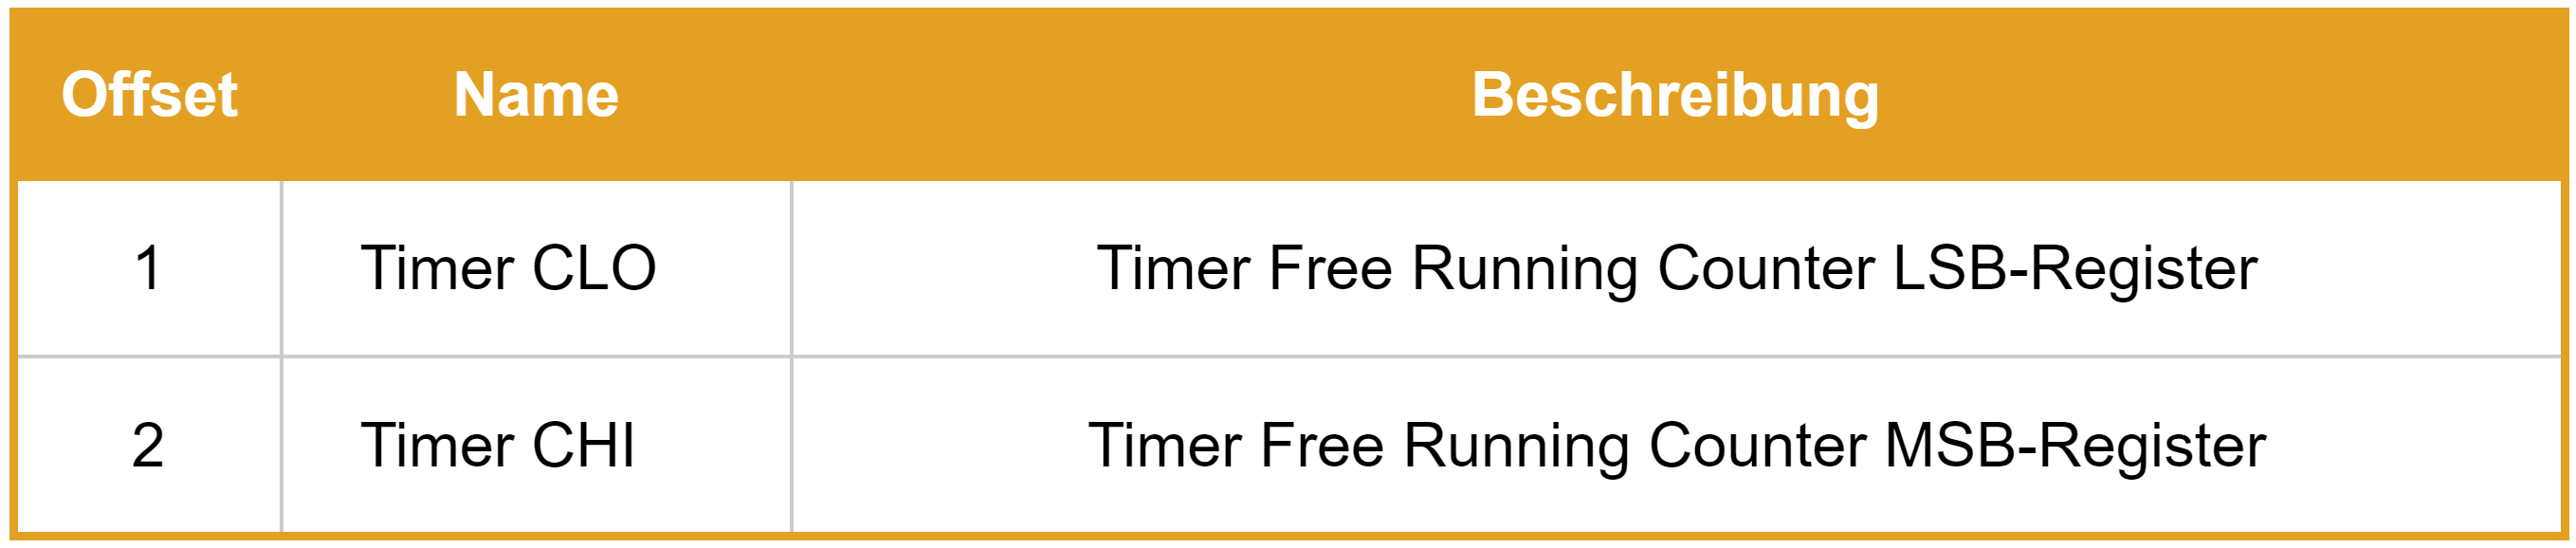
\includegraphics[width=\textwidth]{img/timer_table.png}
\begin{center}\raisebox{9mm}{Abbildung 7: Register des Timer-Controllers (Eigene Darstellung)}\end{center}
\begin{minted}{c++}
class Timer {
    bool paused;
    unsigned int val;
    unsigned int started;
    volatile unsigned int* reg;
public: 
\end{minted}
\vspace{-2mm}
Die Klasse enthält vier Variablen im private-Bereich: 
\begin{compactitem}
\item \textit{paused}, eine Boolean die darstellt, ob der Timer pausiert ist
\item \textit{val}, eine unsigned Integer, die den aktuellen Wert darstellt
\item \textit{started}, eine unsigned Integer, die den Startzeitpunkt speichert
\item \textit{reg}, ein volatile unsigned int*-Pointer, welcher auf die Grundadresse des Timer-Registers zeigt
\end{compactitem}
\begin{minted}{c++}
    Timer() {
        reg = (volatile unsigned int*) 0x20003000;
        val = 0;
        started = 0;
        paused = true;
    }
\end{minted} 
\vspace{-2mm}
Der Konstruktor setzt den Pointer \textit{reg} auf die Adresse 0x20003000, sowie die Variablen \textit{val} und \textit{started} auf 0 und die Boolean \textit{paused} auf false.\\\\\\
\begin{minted}{c++}
    void start() {
        started = reg[1];
        paused = false;
        val = 0;
    }
\end{minted}
\vspace{-2mm}
Die Funktion \textit{start} startet den Timer, indem sie den Wert des Free-Running-Counters aus dem Timer CLO-Register in \textit{started} speichert und \textit{paused} auf false sowie \textit{val} auf 0 setzt.\\
\begin{minted}{c++}
    void stop() {
        paused = true;
        val += reg[1] - started;
        started = 0;
    }
\end{minted}
\begin{minted}{c++}
    void pause() {
        paused = true;
        val += reg[1] - started;
        started = 0;
    }
\end{minted}
\vspace{-2mm}
Die Funktion \textit{stop} stoppt den Timer, indem sie \textit{paused} auf false setzt. Anschließend wird der aktuelle Wert, welcher die Differenz des Counters und \textit{started} ist, zu dem Wert in \textit{val} addiert. Als nächstes wird \textit{started} auf 0 gesetzt. Die Funktion \textit{pause} funktioniert gleich und ist somit nur eine Alternative zu \textit{stop}.\\
\begin{minted}{c++}
    void resume() {
        if(!paused) return;
        paused = false;
        started = reg[1];
    }
\end{minted}
\vspace{-2mm}
Während bei der Funktion \textit{start} der Wert von \textit{val} auf 0 gesetzt wird, wird dieser bei der Funktion \textit{resume} nicht verändert. Somit ermöglicht \textit{resume} das Fortsetzen eines pausierten Timers. Die if-Abfrage verhindert, dass ein aktiver Timer fortgesetzt wird.\\
\begin{minted}{c++}
    bool isRunning() {
        return !paused;
    }
\end{minted}
\vspace{-2mm}
Die Funktion isRunnung liefert den invertierten Wert der Boolean paused zurück, somit kann ermittelt werden, ob der Timer gerade aktiv ist.\\
\begin{minted}{c++}
    unsigned int get() {
        return (val + paused?0:(reg[1] - started)) / 1000000;
    }
\end{minted}
\begin{minted}{c++}
    unsigned int get_ms() {
         return (val + paused?0:(reg[1] - started)) / 1000;
    }
\end{minted}
\begin{minted}{c++}
    unsigned int get_us() {
         return val + paused?0:(reg[1] - started);
    }
\end{minted}
\vspace{-2mm}
Die Funktionen \textit{get}, \textit{get\_ms} und \textit{get\_us} liefern den aktuellen Wert des Timers zurück, indem der gespeicherte Wert in \textit{val} mit dem aktuellen Wert addiert wird, so fern der Timer gerade aktiv ist. Ansonsten wird nur der Wert aus \textit{val} zurückgeliefert. Bei \textit{get} wird der Wert durch 1000000 dividiert, um diesen in Sekunden umzuwandeln, bei \textit{get\_ms} durch 1000, um diesen in Millisekunden umzuwandeln.\\
\begin{minted}{c++}
void wait(unsigned int seconds) {
    seconds = 
        (seconds * 1000000) + *((volatile unsigned int*) 0x20003004);
    while(*((volatile unsigned int*) 0x20003004) < seconds);
}
\end{minted}
\begin{minted}{c++}
void wait_ms(unsigned int millis) {
    millis = (millis * 1000) + *((volatile unsigned int*) 0x20003004);
    while(*((volatile unsigned int*) 0x20003004) < millis);
}
\end{minted}
\begin{minted}{c++}
void wait_us(unsigned int micros) {
    micros = micros + *((volatile unsigned int*) 0x20003004);
    while(*((volatile unsigned int*) 0x20003004) < micros);
}
\end{minted}
\vspace{-2mm}
Die Funktionen \textit{wait}, \textit{wait\_ms} und \textit{wait\_us} sind außerhalb der Klasse \textit{Timer} definiert und verzögern das Programm für eine bestimmte Zeit. Jede Funktion nimmt ein Argument vom Typ unsigned int an. Zuerst wird der Zeitpunkt berechnet, an welchem die Verzögerung abgeschlossen ist. Dieser ist die Summe der übergebenen Verzögerung in $\mu$s und dem aktuellen Wert des Timer CLO-Registers, welches auf der Adresse 0x20003004 liegt. Anschließend wird mit einer while-Schleife gewartet, bis der Wert größer oder gleich dem berechneten Zeitpunkt ist.
\subsection{PWM}
Die PWM-Controller des Raspberry Pi werden über die Klasse \textit{PWM} gesteuert. GPIO 12 und 13 sind mit Kanal 1 und 2 des PWM-Controllers verbunden und können über diesen als PWM-Output genutzt werden. Um PWM nutzen zu können, muss zuerst der Clock-Manager richtig konfiguriert werden. Die Register sind folgendermaßen angeordnet:\\\\
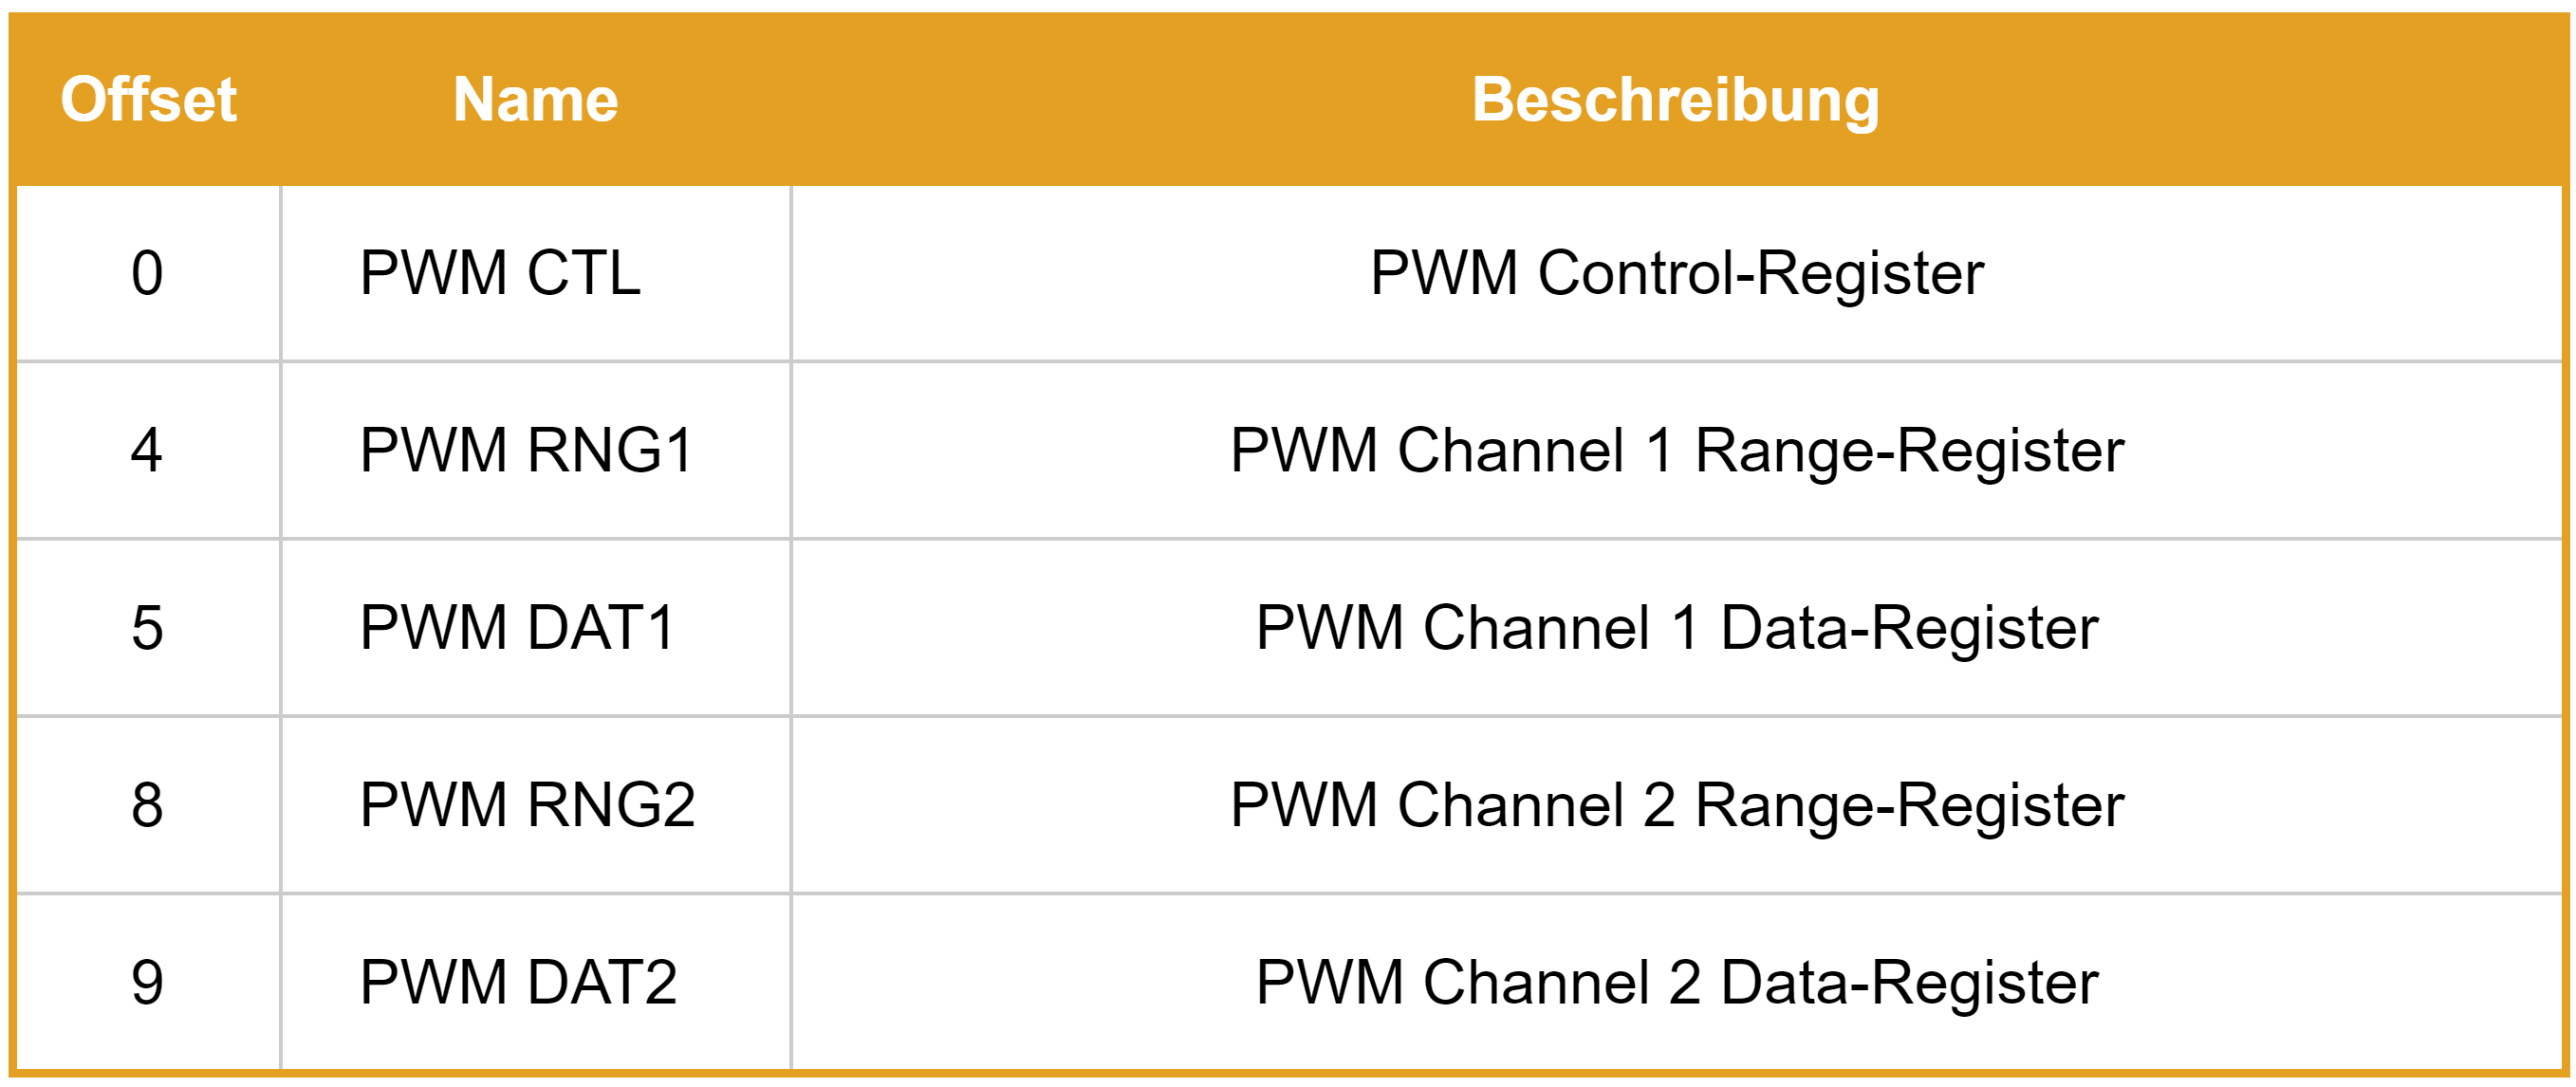
\includegraphics[width=\textwidth]{img/pwm_table.png}
\begin{center}\raisebox{9mm}{Abbildung 8: Register des PWM-Controllers (Eigene Darstellung)}\end{center}
\begin{minted}{c++}
#include "GPIO.hpp"

class PWM {
    char channel;
    volatile unsigned int* reg;
public:
\end{minted}
\vspace{-2mm}
Die Klasse \textit{PWM} enthält einen char, welcher den aktuellen Kanal speichert sowie einen volatile unsigned int*-Pointer, welcher auf die Grundadresse der PWM-Register zeigt. Der Import der Klasse GPIO wird für das Konfigurieren der GPIOs benötigt.\\
\begin{minted}{c++}
    PWM() {}
\end{minted}
\begin{minted}{c++}
    PWM(char channel) {
        this->reg = (unsigned int*) 0x2020C000;
        this->channel = (channel==1) ? 1 : 2;
\end{minted}
\vspace{-2mm}
Der Default-Konstruktor dient nur der Erstellung leerer Instanzen, der richtige Konstruktor nimmt ein Argument von Typ char an, welcher den PWM-Kanal definiert. Als erstes setzt der Konstruktor \textit{reg} auf die Grundadresse der PWM-Register, 0x2020C000. Anschließend wird die Variable \textit{channel} gemäß dem Argument gesetzt. Der Wert 1 resultiert in Channel 1, alles andere wird zu Channel 2.\\
\begin{minted}{c++}        
        volatile unsigned int* clock = (unsigned int*) 0x201010A0;
        clock[1] = (0x5a << 24)  (8 << 12);
        clock[0] = (0x5a << 24)  (1 << 4)  0x01;
\end{minted}   
\vspace{-2mm}
Als nächstes wird ein volatile unsigned int*-Pointer erstellt, welcher auf die Grundadresse des Clock Managers, 0x201010A0, zeigt. Nun wird im Clock Manager die Geschwindigkeit der Clock festgelegt, indem in das Clock Divider-Register, welches einen Offset 1 hat, die Zahl 8 auf die Bits 12-23 geschrieben wird. Weiters muss in jedes Clock Manager-Register in die obersten acht Bits der Wert 0x5A geschrieben werden, damit überhaupt ein Zugriff möglich ist. Danach wird die Clock gestartet, indem in das Clock Control-Register, welches einen Offset von 0 hat, eine 1 auf das fünfte Bit geschrieben wird. Gleichzeitig wird die Quelle der Clock auf den internen Schwingquarz gesetzt, indem eine 1 auf das erste Bit geschrieben wird.\\
\begin{minted}{c++}
        GPIO(this->channel + 11,GPIO::ALT0);
        reg[0] = (0x81) << (this->channel == 1 ? 0 : 8);
        reg[this->channel * 4] = 1000;
    } 
\end{minted}
\vspace{-2mm}
Nach dem Einrichten der Clock wird der entsprechende GPIO auf die ALT0-Funktion gesetzt. Danach wird im PWM CTL-Register der Wert 0x81 je nach Channel auf das erste oder zweite Byte geschrieben. Abschließend wird das PWM RNGx-Register, welches je nach Channel einen Offset von 4 oder 8 hat, mit dem Wert 1000 beschrieben. Dieses Register gibt die Auflösung des PWM-Signals an, der Wert 1000 resultiert in 1000 möglichen Stufen.\\
\begin{minted}{c++}
    void set(double value) {
        value = value > 1.0 ? 1.0 : (value < 0.0 ? 0.0 : value);
        reg[this->channel * 4 + 1] = value * 1000.0;  
    }
\end{minted}
\vspace{-2mm}
Um ein PWM-Signal zu generieren, wird die Funktion \textit{set} verwendet. Als Argument wird eine Variable vom Typ double übergeben, welche einen Wertebereich zwischen 0.0 und 1.0 haben darf. Sollte der Wert außerhalb dieses Bereiches liegen, wird er automatisch korrigiert. Anschließend wird der Wert mit 1000 multipliziert und in das PWM DATx-Register geschrieben, welches je nach Channel einen Offset von 5 oder 9 hat.
\subsection{UART} 
Der UART-Controller des Raspberry Pi wird mit der Klasse \textit{UART} gesteuert und ermöglicht die Verbindung von UART-Geräten mit dem Board. Ebenfalls kann UART mit einen UART/TTY-to-USB-Wandler als Debug-Schnittstelle zum PC genutzt werden. Auf der Platine sind nur die TX- und RX-Pins in Verwendung, die RTS- und CTS-Pins erfüllen andere Funktionen. Der UART-Controller besitzt zwei FIFO-Buffer für Kommunikationen mit mehreren Bytes. Die Register sind folgendermaßen angeordnet:\\
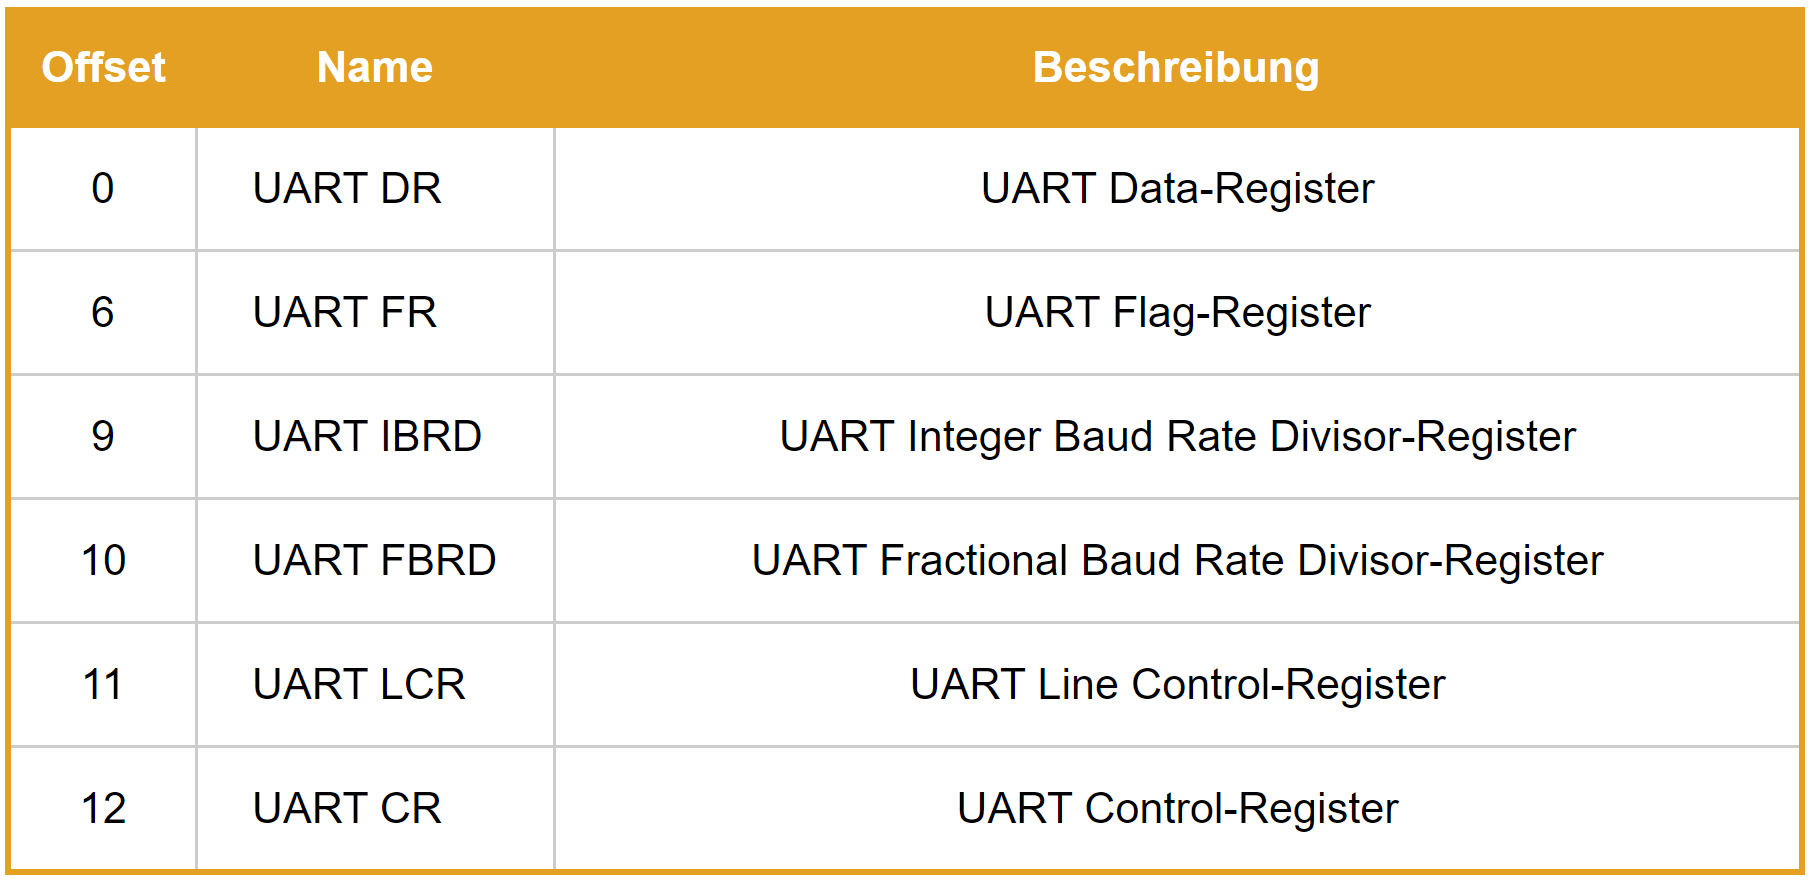
\includegraphics[width=\textwidth]{img/uart_table.png}
\begin{center}\raisebox{9mm}{Abbildung 9: Register des UART-Controllers (Eigene Darstellung)}\end{center}
\begin{minted}{c++}
#include "GPIO.hpp"

class UART {
    volatile unsigned int* reg;
public:
\end{minted}
\vspace{-2mm}
Die Klasse UART enthält nur eine Variable im private-Bereich, einen volatile unsigned int*-Pointer, welcher auf die Grundadresse der UART-Register, 0x20201000 zeigt.\\
\begin{minted}{c++}
    UART() {
        reg = (unsigned int*) 0x20201000;
        GPIO(14, GPIO::ALT0);
        GPIO(15, GPIO::ALT0);
        reg[9] = 26;
        reg[10] = 5; 
        reg[11] = (7 << 4);
        reg[12] = (3 << 7)  0x01;
    }
\end{minted}
\vspace{-2mm}
 Als erstes wird im Konstruktor der Pointer \textit{reg} auf die Adresse 0x20201000 gesetzt, die Grundadresse der UART-Register.\\
 Anschließend werden die GPIOs 14 und 15 mit der Alternativen Funktion 0 konfiguriert, um als UART-Pins zu fungieren. Die Frequenz wird mit Hilfe der UART IBRD- und UART FBRD-Register auf eine Baudrate von 115200 angepasst. Als nächstes werden im UART LCR-Register, die FIFOs aktiviert und die Wortlänge auf 8 gesetzt. Dies erfolgt durch das setzen der Bits 4, 5 und 6. Zuletzt werden im UART CR-Register der UART Controller, der Reciever und der Transmitter aktiviert, indem die Bits 0, 7 und 8 auf 1 gesetzt werden.\\
\begin{minted}{c++}
    void print(char* string) {
        while(*string) {
            while(reg[6] & (1 << 5));
            reg[0] = *(string++);
        }
    }
\end{minted}
\vspace{-2mm}
Die Funktion \textit{print} nimmt einen String als Argument an, welcher dann über UART geschrieben wird. Mit einer while-Schleife wird jedes Zeichen nacheinander abgearbeitet: Zuerst wird mit einer while-Schleife gewartet, falls der Transfer-FIFO voll ist, dies wird an Bit 5 im UART FR-Register erkannt. Anschließend wird das Zeichen in den FIFO geladen, indem es auf die niedrigsten acht Bits des UART DR-Registers geschrieben wird.\\
\begin{minted}{c++}
    char* read(int bytes) {
        char data[bytes];
        if(reg[6] & (1 << 4)) return 0;
        for(int i = 0; !(reg[6] & (1 << 4)); i++) {
            data[i] = reg[0] & 0xFF;
        } char* ptr = data;
        return ptr;
    }
\end{minted}
\vspace{-2mm}
Die Funktion \textit{read} liefert einen char*-Pointer zurück, welcher auf die empfangenen Daten zeigt und nimmt die Anzahl der auszulesenden Byte als Argument vom Typ int an.\\
Zuerst wird mit einer if-Abfrage überprüft, ob der Recieve-FIFO leer ist. Dies kann an Bit 4 im UART FR-Register, welches einen Offset von 6 hat, erkannt werden. Wenn der FIFO leer ist, wird ein Null-Pointer zurückgegeben. Ansonsten wird mit einer for-Schleife, mit der Bedingung, dass der FIFO nicht leer ist, das Array \textit{data} befüllt. Der aktuelle Index wird mit dem Wert der untersten acht Bits des UART DR-Registers beschrieben. Nach der Befüllung des Arrays wird ein Pointer, welcher auf das Array zeigt, erstellt und zurückgegeben.
\subsection{SPI}
Das SPI-Interface des Raspberry Pi wird über die Klasse \textit{SPIDevice} gesteuert. Es kann als Master und als Slave verwendet werden, auf dieser Platine kommt jedoch nur die Master-Funktion zum Einsatz. Der SPI-Master enthält wie der UART-Controller auch zwei FIFO-Buffer, einen für zu sendende und einen für empfangene Daten. Die Register sind folgendermaßen angeordnet:\\\\
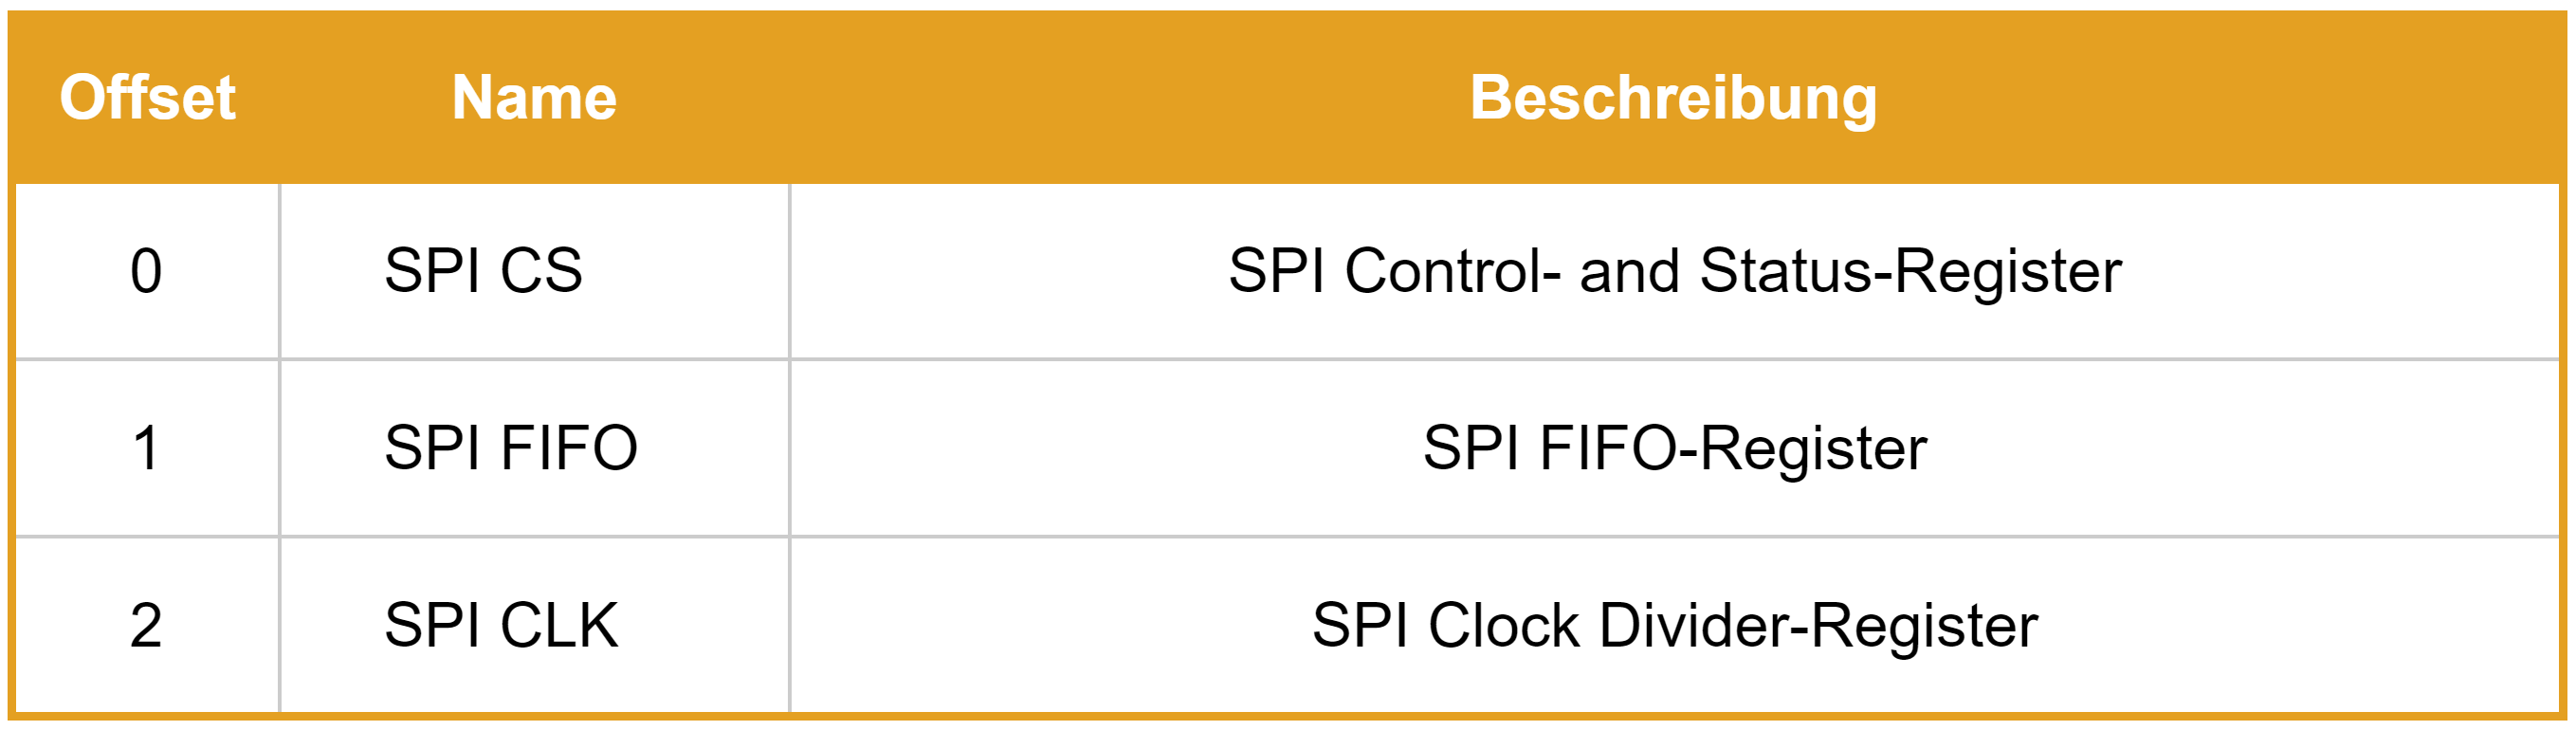
\includegraphics[width=\textwidth]{img/spi_table.PNG}
\begin{center}\raisebox{9mm}{Abbildung 10: Register des SPI-Controllers (Eigene Darstellung)}\end{center}
\newpage
\begin{minted}{c++}
#include "GPIO.hpp"

class SPIDevice {
    char cs;
    char mode;
    bool pulse;
    unsigned int freq;
    volatile unsigned int* reg;
public:
\end{minted}
\vspace{-2mm}
Die Klasse enthält fünf Variablen im private-Bereich:
\begin{compactitem}
\item \textit{cs}, ein Character, welcher die ID des CS-Pins speichert.
\item \textit{mode}, ein Character, welcher den SPI-Mode(0 - 3) speichert.
\item \textit{pulse}, eine Boolean, die darstellt, ob der CS-Pin nach jedem Byte kurz auf High geht.
\item \textit{freq}, eine unsigned Integer, in der die Frequenz gespeichert wird.
\item \textit{reg}, einen volatile unsigned int*-Pointer, welcher auf die Grundadresse der SPI-Register zeigt.
\end{compactitem} Der Import der Klasse GPIO wird zur Steuerung der Chip-Select-Pins benötigt.\\
\begin{minted}{c++}
    SPIDevice() {}
\end{minted}
\begin{minted}{c++}
    SPIDevice(char cs, char mode, bool pulse, unsigned int freq) {
        this->reg = (unsigned int*) 0x20204000;
        this->cs = cs;
        this->mode = mode;
        this->pulse = pulse;
        this->freq = (125000000/freq)*2;
        GPIO(9, GPIO::ALT0);
        GPIO(10, GPIO::ALT0);
        GPIO(11, GPIO::ALT0);
        GPIO(cs, GPIO::OUTPUT).setLevel(true);
    }
\end{minted}
\vspace{-2mm}
Die Klasse hat zwei Konstruktor, der Default-Konstruktor ist jedoch nur zur Erstellung leerer Instanzen gedacht.\\
Der richtige Konstruktor nimmt vier Argumente an, welche den Variablen im private-Bereich der Klasse entsprechen. Als erstes wird \textit{reg} auf die Grundadresse der SPI-Register, 0x20204000, gesetzt. Anschließend wird der Wert der Argumente \textit{cs}, \textit{mode} und \textit{pulse} in die gleichnamigen Variablen kopiert. Da die Frequenz in Clock-Ticks angegeben werden muss, muss sie zuerst mit folgender Formel umgerechnet werden, bevor sie in \textit{freq} gespeichert wird: $freq_{ticks} = \frac{125 Mhz}{freq_{Hz}} * 2$. Als nächstes werden die GPIOs 9, 10 und 11, welche mit dem SPI-Controller verbunden sind, auf die Alternative Funktion 0 gesetzt, um die SPI-Funktion zu aktivieren. Zuletzt wird der CS-Pin als Output konfiguriert und auf HIGH gesetzt.\\
\begin{minted}{c++}
    unsigned char transfer(unsigned char data) {
        GPIO(cs).setLevel(false);
        reg[0] = (mode << 2);
        reg[2] = freq;
        reg[0] = (3 << 4)  (1 << 7);
\end{minted}
\vspace{-2mm}
Die Funktion \textit{transfer} sendet ein Byte, welches als Argument vom Typ unsigned Character
übergeben wird und liefert die Antwort ebenfalls als unsigned Character zurück. Zuerst setzt die Funktion den CS-Pin auf LOW, danach wird im SPI Control-and-Status-Register, welches einen Offset von 0 hat, der Wert der Variable \textit{mode} auf die Bits 2 bis 3 geschrieben. Anschließend wird in das Clock-Divider-Register, welches einen Offset von 2 hat, der Wert der Variable \textit{freq} geschrieben, um die Übertragungsgeschwindigkeit zu setzen. Nun wird auf die Bits 4, 5 und 7 im SPI CS-Register eine 1 geschrieben, welche den FIFO leert und die Kommunikation startet.\\\\\\
\begin{minted}{c++}
        reg[1] = data;
        while(!(reg[0] & (1<<16)));
        GPIO(cs).setLevel(true);
        return reg[1];
    }
\end{minted}
\vspace{-2mm}
Danach wird in das SPI FIFO-Register das zu übertragende Byte geschrieben, welches dann gesendet wird. Mit einer while-Schleife wird nun gewartet, bis die Kommunikation abgeschlossen wurde. Dies erfolgt über die Abfrage von Bit 16 im SPI CS-Register, das bei Ende der Kommunikation den Wert 1 annimmt. Abschließend wird der CS-Pin wieder auf HIGH gesetzt und das empfangene Byte aus dem SPI FIFO-Register gelesen und zurückgegeben.\\
\begin{minted}{c++}
    unsigned char* transfer(unsigned char* data, int len) {
        unsigned char out[len];
        if(pulse) {
            for(int i = 0; i < len; i++) out[i] = transfer(data[i]);
        } 
\end{minted}
\vspace{-2mm}
Eine Kommunikation über mehrere Bytes erfolgt über die Funktion \textit{transfer}, welche einen Pointer sowie einen Integer als Argumente annimmt und einen unsigned char*-Pointer zurückliefert. Die Übergabe der Daten erfolgt mittels char-Pointer zu einem Array, welches die Länge \textit{len} hat.\\
Der zurückgegebene Pointer zeigt auf ein Array mit Länge \textit{len}, in welchem die empfangenen Bytes gespeichert sind. Als erstes wird das Ausgabe-Array \textit{out} mit der Länge \textit{len} erstellt, danach wird mit einer if-Abfrage unterschieden, ob \textit{pulse} true oder false ist. Wenn \textit{pulse} true ist, wird mit einer for-Schleife jedes Byte einzeln über die Funktion \textit{transfer} verarbeitet und der Rückgabewert an der richtigen Stelle in \textit{out} gespeichert.\\
\begin{minted}{c++}
        else {
            GPIO(cs).setLevel(false);
            reg[0] = (mode << 2);
            reg[2] = freq;
            reg[0] = (3 << 4)  (1 << 7);
            for(int i = 0; i < len; i++) reg[1] = data[i];
            while(!(reg[0] & (1<<16)));
            for(int i = 0; i < len; i++) out[i] = reg[1];
            GPIO(cs).setLevel(true);
        } 
\end{minted}
\vspace{-2mm}
Wenn \textit{pulse} jedoch false ist, findet der gleiche Vorgang wie in der Funktion \textit{transfer} statt, jedoch werden statt einem einfachen Schreibvorgang in das SPI FIFO-Register alle Bytes mit einer for-Schleife nacheinander hineingeschrieben. Beim Auslesen der empfangenen Daten werden wieder mit Hilfe einer for-Schleife die Bytes aus dem FIFO gelesen und an der richtigen Stelle im Array \textit{out} gespeichert.\\
\begin{minted}{c++}
         unsigned char* ptr = out;
        return ptr;
    }
\end{minted}
\vspace{-2mm}
Da in C++ keine Arrays als Argumente oder Rückgabewerte übergeben werden sollen, muss ein Pointer, welcher auf das Array \textit{out} zeigt, erstellt und von der Funktion zurückgeben werden.\\
\begin{minted}{c++}
    void setFrequency(unsigned int freq) {
        this->freq = (125000000/freq)*2;
    }
\end{minted}
\begin{minted}{c++}
    void setMode(char mode) {
        this->mode = mode;
    }
\end{minted}
\begin{minted}{c++}
    void setPulse(bool pulse) {
        this->pulse = pulse;
    }
\end{minted}
\vspace{-2mm}
Die Funktion \textit{setFrequency} nimmt ein Argument vom Typ unsigned Integer an und berechnet den Wert der Variable \textit{freq} mit derselben Formel wie im Konstruktor.
Die Funktionen \textit{setMode} und \textit{setPulse} nehmen je eine Argument an und kopieren dieses in die gleichnamige Variable.\\
\subsection{I2C}
Der I2C-Controller des Raspberry Pi wird mit der Klasse \textit{I2CDevice} gesteuert, jedoch nur als I2C-Master, da auf der Platine keine andere Verwendung vorhergesehen ist. Der I2C-Controller enthält wie der SPI-Controller und der UART-Controller auch zwei FIFO-Buffer, welche eine Kommunikation mit mehreren Bytes ermöglichen. Die Register sind folgendermaßen strukturiert:\\\\
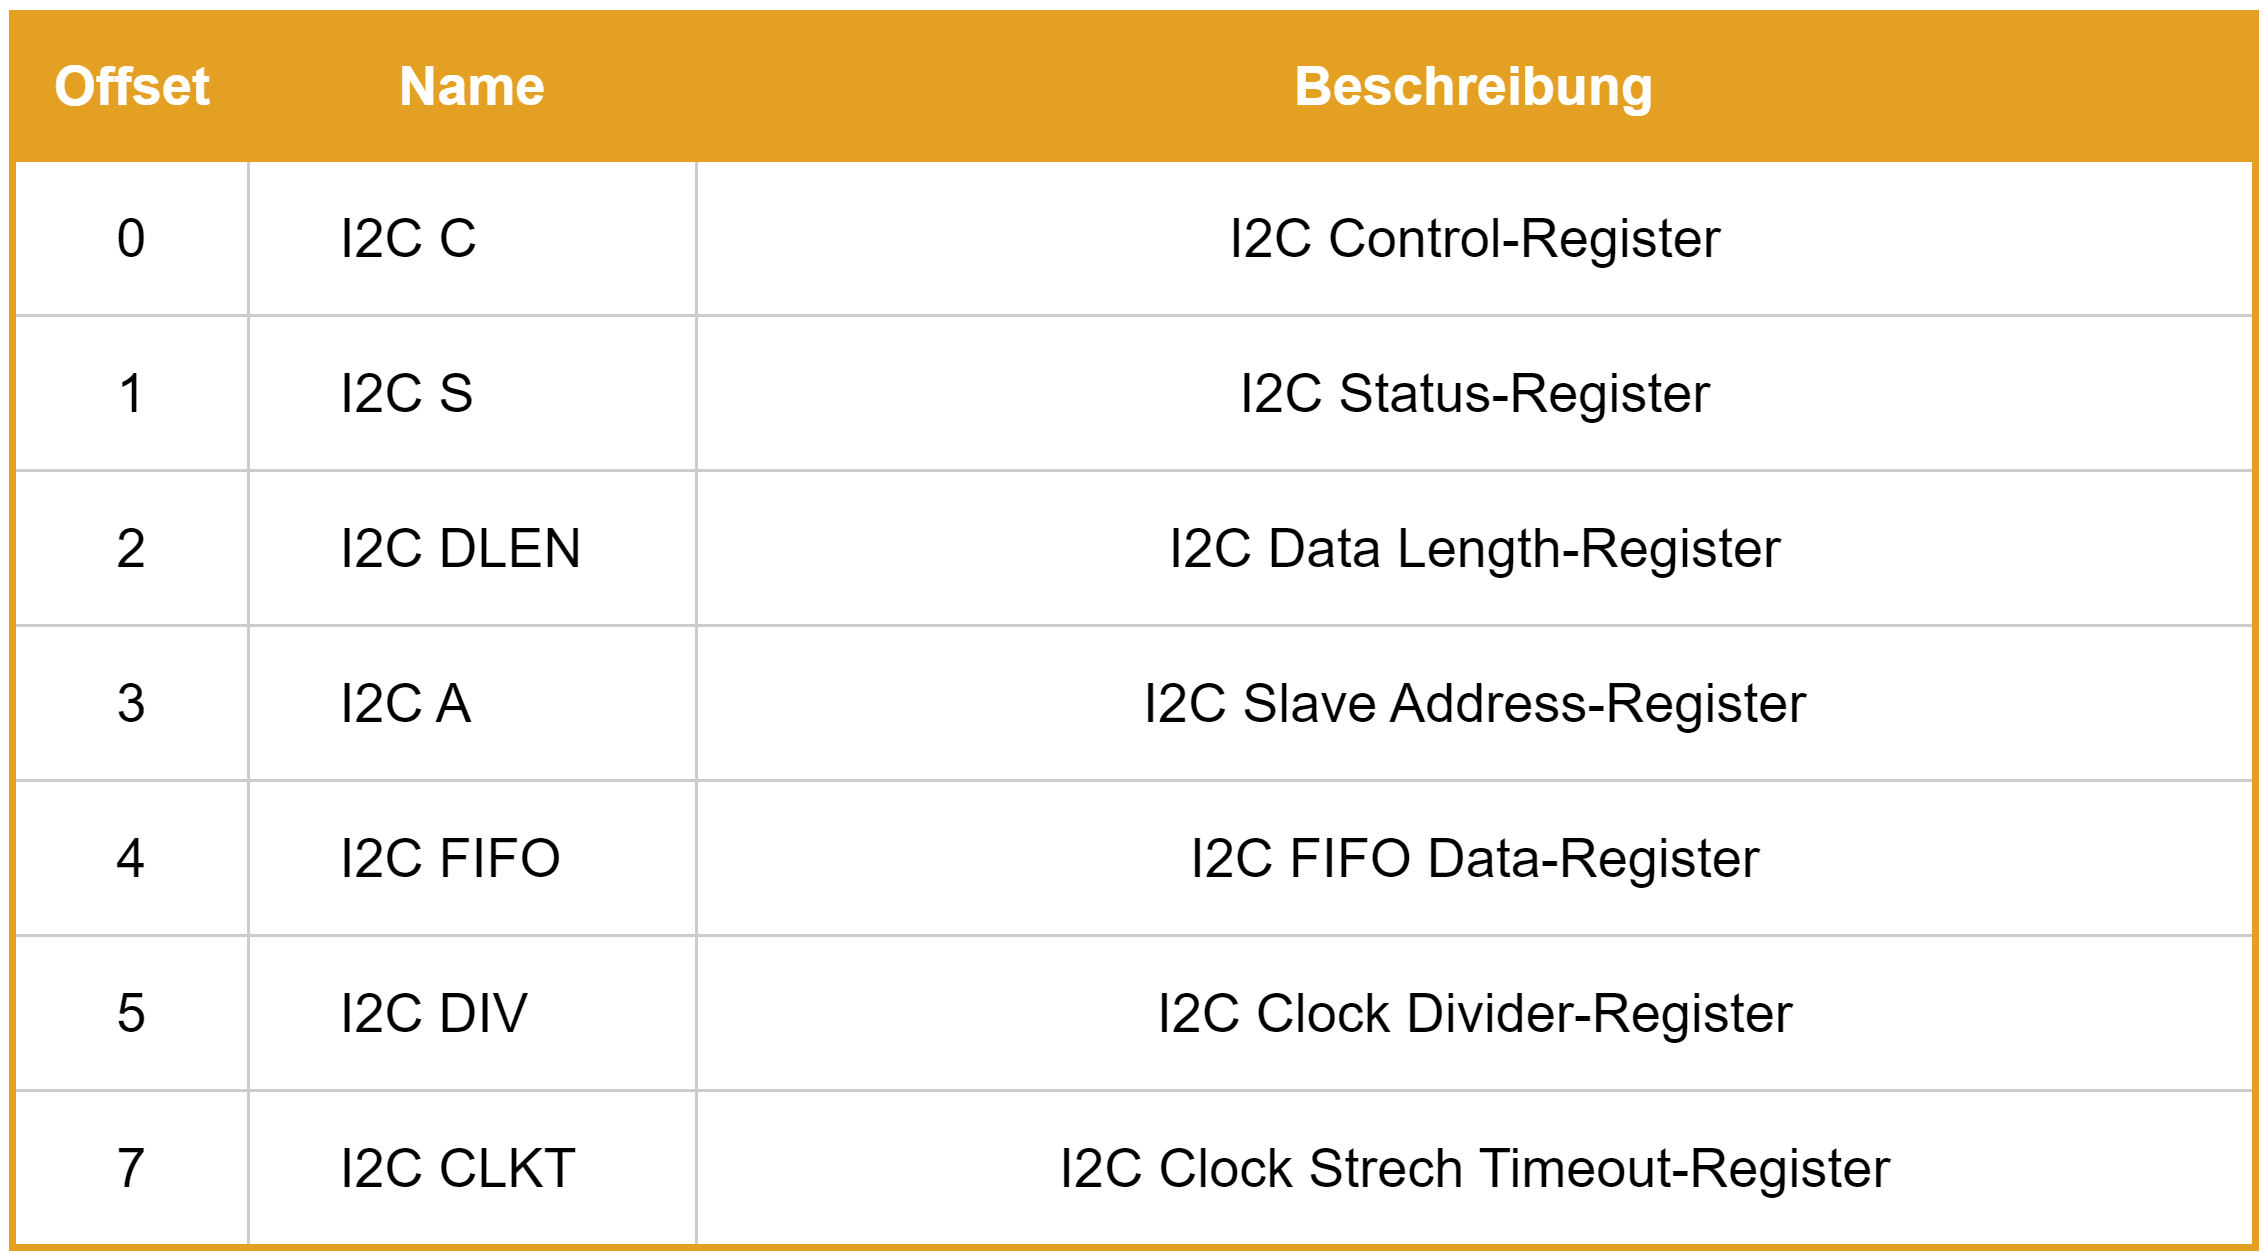
\includegraphics[width=\textwidth]{img/i2c_table.png}
\begin{center}\raisebox{9mm}{Abbildung 11: Register des I2C-Controllers (Eigene Darstellung)}\end{center}
\begin{minted}{c++}
#include "GPIO.hpp"

class I2CDevice {
    char address;
    int csto;
    unsinged int freq;
    volatile unsigned int* reg;
public:
\end{minted}
\vspace{-2mm}
Die Klasse enthält vier Variablen im private-Bereich:
\begin{compactitem}
\item \textit{address}, ein Character, welcher die 7-Bit-Adresse des Slaves speichert.
\item \textit{csto}, eine Integer, die den Clock Stretch Timeout speichert.
\item \textit{freq}, eine unsigned Integer, in der die Frequenz gespeichert wird.
\item \textit{reg}, einen volatile unsigned int*-Pointer, welcher auf die Grundadresse der I2C-Register zeigt.
\end{compactitem}
\begin{minted}{c++}
    I2CDevice() {}
\end{minted}
\begin{minted}{c++}
    I2CDevice(char address, unsigned int freq, int csto) {
        this->reg = (unsigned int*) 0x20804000;
        this->address = address & 0x7F;
        this->freq = (125000000/freq)*2;
        this->csto = csto ? csto : 0x40;
        GPIO(2, GPIO::ALT0);
        GPIO(3, GPIO::ALT0);
        reg[0] = (1 << 15);
    }
\end{minted}
\vspace{-2mm}
Der Default-Konstruktor dient nur zur Erstellung leerer Instanzen, die nicht funktionsfähig sind. Der richtige Konstruktor nimmt als Argumente die I2C-Adresse des Slaves, die gewünschte Frequenz und den Clock Stretch Timeout an. Als erstes wird der Pointer \textit{reg} auf die Grundadresse 0x20804000 gesetzt, anschließend wird der Wert des ersten Arguments in die Variable \textit{address} übertragen, wobei nur die untersten sieben Bits erhalten werden.\\
Als nächstes wird die Frequenz mit der Formel $freq_{ticks} = \frac{125 Mhz}{freq_{Hz}} * 2$ in Clock-Ticks umgewandelt und in \textit{freq} gespeichert. Für den Clock Stretch Timeout wird der Wert des dritten Arguments abgespeichert, wenn dieser nicht 0 ist, ansonsten wird der Wert 0x40 gespeichert. Danach werden die GPIOs 2 und 3 mit der alternativen Funktion 0 konfiguriert, bevor im I2C C-Register, eine 1 auf das Bit 15 geschrieben wird. Dadurch wird der I2C-Controller aktiviert und kann über die GPIOs 2 und 3 kommunizieren.\\
\begin{minted}{c++}
    void setFrequency(unsigned int freq) {
        this->freq = (125000000/freq)*2;
    }
\end{minted}
\begin{minted}{c++}
    void setClockStretchTimeout(int csto) {
        this->csto = csto ? csto : 0x40;
    }
\end{minted}
\vspace{-2mm}
Die Funktionen \textit{setFrequency} und \textit{setClockStretchTimeout} nehmen je ein Argument vom Typ Integer ab, wobei dieser bei \textit{setFrequency} jedoch eine unsigned Integer ist. Der übergebene Wert wird gleich wie im Konstruktor umgerechnet und in der entsprechende Variable abgespeichert. Diese beiden Funktionen dienen zur Veränderung der ursprünglichen Werte.\\
\begin{minted}{c++}
    void write(char* data, int len) {
        reg[2] = len;
        reg[3] = address;
        for(int i = 0; i < len; i++) reg[4] = data[i];
        reg[5] = freq;
        reg[7] = csto;
        reg[0] &= ~(1);
        reg[0] = (1 << 7);
        while(!(reg[1] & 0x202));
        reg[1] = 0x202;
    }
\end{minted}
\vspace{-2mm}
Die Funktion \textit{write} nimmt zwei Argumente an, einen char*-Pointer und einen Integer, wobei der Pointer auf ein char-Array zeigen muss und das zweite Argument dessen Länge entsprechen muss. Zuerst wird in das I2C DLEN-Register der Wert des zweiten Arguments gespeichert. Anschließend wird in das I2C A-Register die Adresse des Slaves geschrieben. Als nächstes wird jedes Byte des übergebenen char-Arrays in das I2C FIFO-Register kopiert und das I2C DIV-Register mit dem Wert von \textit{freq} befüllt sowie das I2C CLKT-Register mit dem Wert der Variable \textit{csto} beschrieben. Danach wird im I2C C-Register das Bit 0 auf 0 gesetzt, um den Modus auf "Write" zu setzen, anschließend wird durch eine 1 auf dem Bit 7 die Übertragung gestartet. Nun wird mit Hilfe einer while-Schleife gewartet, bis entweder das Bit 9 oder Bit 1 im I2C S-Register auf 1 gehen, was ein Ende der Übertragung markiert. Anschließend werden beide Bits wieder auf 1 gesetzt, um diese zurückzusetzen.\\
\begin{minted}{c++}
    char* read(int len) {
        char out[len];
        reg[2] = len;
        reg[3] = address;
        reg[5] = freq;
        reg[7] = csto;
        reg[0] = (1 << 7)  1;
        while(!(reg[1] & 0x102));
        reg[1] = 0x102;
        for(int i = 0; i < len; i++) out[i] = reg[4];
        char* ptr = out;
        return ptr;
    }
\end{minted}
\vspace{-2mm}
Die Funktion \textit{read} nimmt einen Integer als Argument an, welcher die Anzahl der zu lesenden Bytes festlegt und liefert einen char*-Pointer auf ein entsprechend großes char-Array zurück. Als Erstes wird das char-Array \textit{out} mit der Größe des Arguments erstellt, in welchem die empfangenen Daten gespeichert werden.\\
Als nächstes wird in das I2C DLEN-Register der Wert des Arguments gespeichert und in das I2C A-Register die Adresse des Slaves geschrieben. Danach wird das I2C DIV-Register mit dem Wert der Variable \textit{freq} befüllt sowie das I2C CLKT-Register mit dem Wert der Variable \textit{csto} beschrieben. Um den Lesevorgang zu starten wird im I2C C-Register das Bit 1 auf 1 gesetzt, um den Modus auf "Read" zu setzen, anschließend wird durch eine 1 auf Bit 7 die Kommunikation gestartet. Nachdem mit einer while-Schleife gewartet wurde, bis entweder das Bit 9 oder Bit 1 im I2C S-Register den Wert 1 angenommen haben und somit die Kommunikation beendet wurde, werden die beiden Bits mit 1 beschrieben, um diese zurückzusetzen. Als nächstes wird mit einer for-Schleife das Array \textit{out} mit Daten aus dem I2C FIFO-Register befüllt, in welchem die empfangenen Daten liegen. Abschließend wird ein Pointer zu \textit{out} erstellt und zurückgegeben.\\
\begin{minted}{c++}
    char* command(char* data, int wlen, int rlen) {
        reg[2] = wlen;
        reg[3] = address;
        for(int i = 0; i < wlen; i++) reg[4] = data[i];
        reg[5] = freq;
        reg[7] = csto;
        reg[0] &= ~(1);
        reg[0] = (1 << 7);
        while(!(reg[1] & 1));
        char out[rlen];
        reg[2] = rlen;
        reg[0] = (1 << 7)  1;
        while(!(reg[1] & 0x102));
        reg[1] = 0x102;
        for(int i = 0; i < rlen; i++) out[i] = reg[4];
        char* ptr = out;
        return ptr;
    }
\end{minted}
\vspace{-2mm}
Die Funktion \textit{command} ist eine Kombination aus \textit{write} und \textit{read}, welche auf dem Repeated Start Feature des I2C-Busses basiert. Die Funktion nimmt drei Argumente an: Einen char*-Pointer für die zu sendenden Daten, sowie eine Integer, welche die Anzahl der zu sendenden Bytes festlegt und eine Integer, welche die Anzahl der auszulesenden Bytes bestimmt. Die Register werden gleich wie in der Funktion \textit{write} beschrieben, danach wird jedoch gewartet, bis im I2C S-Register das Bit 0 auf 1 geht, was einen Kommunikationsstart symbolisiert. Während der Schreibvorgang aktiv ist, wird nun der Lesevorgang gestartet, welcher zu einem Repeated Start führt. Daher wird nun der gleiche Code wie in der Funktion \textit{read} ausgeführt, jedoch müssen das I2C A-, I2C DIV-, und das I2C CLKT-Register nicht erneut beschrieben werden, da der Wert gleich bleibt. 
\newpage\section{ATmega Software}
In diesem Kapitel wird der Code, welcher auf dem Subprozessor läuft, beschrieben. Hierbei handelt es sich jedoch nur um Pseudocode, da dies andernfalls den Rahmen der Arbeit sprengen würde.
\subsection{8-Bit AVR Plattform}
Die Programmierung des Subprozessors, einem ATMega644, erfolgt auch in C++. Als 
Entwicklungsumgebung kommt Atmel Studio zum Einsatz, da der avr-gcc-Compiler dort bereits inkludiert ist. Der Sourcecode wird in eine Binärdatei kompiliert, welche dann mit einem AVR-In-System-Programmers auf den ATmega geladen wird. Die Verbindung mit dem ATmega erfolgt über den ISP-Stecker auf der Platine. 
\\\\Der ATMega644 besitzt vier Fuses-Register, über welche ein paar grundlegende Einstellungen vorgenommen werden können: Im Low-Fuse-Register kann die Taktrate gesteuert werden sowie ob ein externer Quarz verwendet wird. Auf der Platine ist ein Full-Swing-Quarz mit einer Taktrate von 20 MHz verbaut, somit soll dieser auch verwendet werden. Die Option "Divide clock by 8 internally" sollte ausgeschaltet werden, damit eine höhere Leistung erreicht werden kann. Im High-Fuse-Register muss SPI aktiviert sein, um eine Kommunikation mit dem Raspberry Pi zu ermöglichen, aber JTAG deaktiviert sein, da das JTAG-Interface ein paar Pins in der Funktionalität einschränkt.
\\\\Weil der ATMega644 ein 8-Bit-Prozessor ist, hat jedes Register eine Größe von 8 Bits. Wenn etwas mehr Bits benötigt, ist es auf mehrere Register aufgeteilt.\\\\
Alle Register sind in der Library von Atmel/Microchip definiert, somit müssen sie nicht über die Speicheradresse adressiert werden. Auch die einzelnen Bits sind bereits mit Namen definiert, was die Programmierung wesentlich erleichtert. 
\subsection{IO}
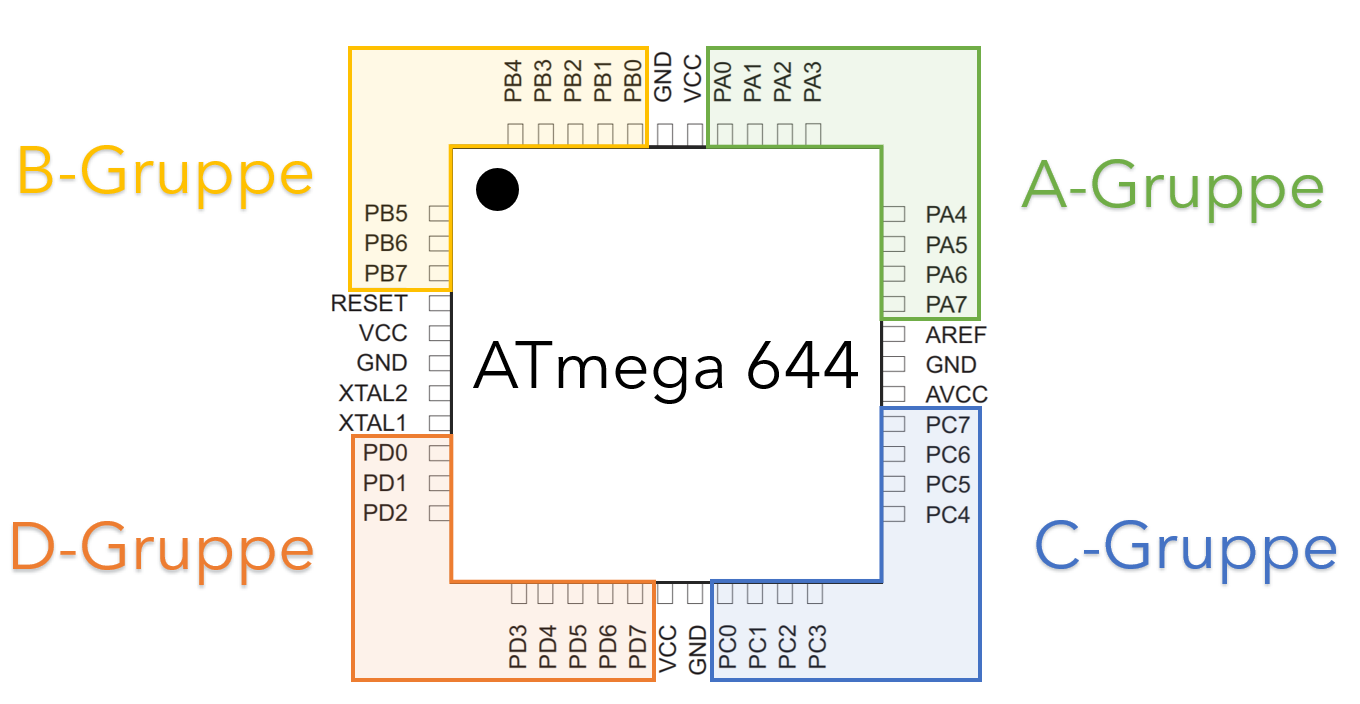
\includegraphics[width=\textwidth]{img/ATmegaPinout.PNG}
\begin{center}
\raisebox{4mm}{Abbildung 12: Pingruppen des ATmega644 in der TQFP-44 Bauform}
\end{center}
Alle 32 ansteuerbaren Pins des ATMega sind in 4 Gruppen aufgeteilt, welche mit A bis D benannt sind. Das Steuern der Pins erfolgt mithilfe der Data-Direction-(DDR), Port-(PORT) und Pin(PIN)-Register, welche pro Gruppe je einmal existieren. Um beispielsweise den Pin B2 als Output zu definieren, muss in das DDRB-Register auf Bit 2 eine 1 geschrieben werden.
\\\\Um einen Pin zwischen Output und Input zu wechseln, wird das DDR-Register genutzt. Wenn auf das entsprechende Bit eine 1 geschrieben wird, ist der Pin ein Output.\\\\
Um einen Output ein- oder auszuschalten wird das PORT-Register genutzt, eine 1 auf dem entsprechendem Bit resultiert in einem logischen HIGH. Sollte der Pin ein Input sein, aktiviert eine 1 im PORT-Register den internen Pull-Up-Widerstand. Um einen Pin auszulesen, muss das entsprechende Bit im PIN-Register gelesen werden, eine 1 signalisiert ein logisches HIGH auf dem Pin.
\subsection{SPI}
Das SPI-Interface des ATmega liegt auf den Pins B4 bis B7, wovon B4 der Chip-Select-, B5 der MOSI-, B6 der MISO und B7 der Clock-Pin ist. Der SPI-Controller kann als SPI Slave sowie als SPI Master genutzt werden, hier auf der Platine ist der ATMega jedoch ein SPI Slave, welcher von dem Raspberry Pi gesteuert wird. Das SPI-Interface besitzt im Gegensatz zum Raspberry Pi keinen Buffer, sondern nur ein 8-Bit Data-Register.
\\\\Zur Initialisierung des SPI-Controllers müssen folgende Schritte erfolgen: Die Pins B4, B5 und B7 müssen als Input konfiguriert sein, B6 jedoch als Output. Anschließend wird in das SPCR-Register, dem SPI-Control-Register, das SPI-Enable- und das SPI-Interrupt-Enable-Bit auf 1 gesetzt. Als nächstes wird in das SPDR-Register, dem SPI-Data-Register, der Wert 0x00 geschrieben. Abschließend werden mit einem Aufruf der Funktion \textit{sei()} der AVR-Library Interrupts aktiviert.
\\\\Wenn Daten empfangen werden, wird die SPI-Interrupt-Routine aufgerufen, welche wie folgt definiert wird: \textit{ISR(SPI\_STC\_vect) \{...\}}. Das empfangene Byte muss zuerst aus dem SPDR-Register ausgelesen werden, anschließend kann eigener Code ausgeführt werden.\\
Um die Antwort auf die nächste Übertragung festzulegen, wird ein Byte in das SPDR-Register geschrieben. Die Interrupt-Routine sollte optimalerweise keine großen Verzögerungen enthalten, da sonst nicht genug Zeit für eine korrekte SPI-Antwort bleibt.
\subsection{ADC}
Jeder der 8 Pins der A-Gruppe ist mit dem Analog-Digital-Wandler verbunden, somit ist auf jedem Pin das Messen der analogen Spannung möglich. Der Analog-Wandler funktioniert mithilfe einer internen Referenzspannung, welche langsam verändert wird und über einen Operationsverstärker ein digitales Signal auslöst. Es kann immer nur ein Kanal gleichzeitig ausgewertet werden, da alle Kanäle mit einem Multiplexer verbunden sind. 
\\\\Die Initialisierung des ADC erfolgt durch folgende Schritte: Als Erstes müssen im ADCSRA-Register das ADC-Enable-, ADC-Interrupt-Enable-, ADC-Start-Conversion- und die drei ADC-Prescaler-Bits auf 1 gesetzt werden. Dies aktiviert den ADC und die dazugehörigen Interrupts und startet eine Messung. Die Taktrate des ADC wird über die drei Prescaler-Bits auf  $\frac{20MHz}{128} = $ 156.25 KHz gesetzt. Optional kann zuvor im ADMUX-Register, dem Multiplexer-Channel-Register, ein Channel ausgewählt werden. Um den Interrupt-Controller zu aktivieren, muss die Funktion \textit{sei()} der AVR-Library aufgerufen werden.
\\\\Sobald die Messung abgeschlossen ist, wird die ADC-Interrupt-Routine aufgerufen, welche mit \textit{ISR(ADC\_vect) \{...\}} definiert wird. Dort müssen zuerst das ADCH- und ADCL-Register gelesen werden, in welchen das Ergebnis der Messung gespeichert ist. Nach der Ausführung von eigenem Code kann eine neue Messung gestartet werden, indem in das ADCSRA-Register das ADC-Start-Conversion-Bit sowie das ADC-Interrupt-Flag-Bit auf 1 gesetzt werden. Im Gegensatz zum SPI-Interrupt dürfen in dieser Interrupt-Routine Verzögerungen verwendet werden.
\subsection{PWM}
Die Erzeugung von PWM-Signalen erfolgt auf dem ATMega mithilfe der internen Clocks, welche einen Vergleichswert nutzen, um den Output auf HIGH oder auf LOW setzen. Der ATmega hat 6 Timer, auf dieser Platine werden nur die Timer 1A, 1B, 2A und 2B genutzt. Der Output des PWM-Signals erfolgt über die Pins D4 - D7, welche dafür als Output konfiguriert werden müssen.
\\\\Die Initialisierung des Timers 1 erfolgt durch das Setzen der Output-Compare-Bits COM1A0 und COM1B0 sowie des WGM0-Bits im Timer 1 Control-Register TCCR1A. Im Register TCCR1B werden das WGM2-Bit sowie das CS1-Bit auf 1 gesetzt. Dies hat zur Folge, dass der Timer im 8-Bit Fast-PWM Modus läuft und bei selben Wert wie im Timer-Compare-Register den dazugehörigen Pin an oder ausschaltet. Durch das CS1-Bit wird der Prescaler der PWM-Frequenz auf den Wert 8 gesetzt. Für Timer 2 ist der Vorgang fast ident, jedoch befindet sich das WGM2-Bit im TCCR2A-Register, statt in dem TCCR2B-Register.
\\\\Um nun ein PWM-Signal zu erzeugen, wird in das entsprechende Output-Compare-Register der Vergleichswert geschrieben. Für Channel 1A ist das Output-Compare-Register das OCR1A-Register.\\
Der Wert 0 im Register resultiert in einem 0\% Duty-Cycle, der Wert 255 in einem 100\% Duty-Cycle. Bei der Verwendung von Motortreibern, wie den VNH7100ASTR, die zwei Motordrehrichtungen unterstützen, müssen zusätzlich die Direction-Pins der Motortreiber richtig angesteuert werden. Dies erfolgt über das ein- oder ausschalten bestimmter Output-Pins des ATMega.
\newpage\section{Ansteuerung von Komponenten}
In diesem Kapitel werden alle Klassen der Library beschrieben, welche zur Steuerung von Komponenten auf der Platine notwendig sind. Zusätzlich dazu wird erklärt, wie eigene Hardware angeschlossen und verwendet werden kann.
\subsection{Status LED}
Die Status LED auf der Platine ist eine Zwei-Farben LED, welche aus einer roten und einer grünen LED besteht, die sich die Kathode teilen. Die grüne LED ist an GPIO 24, die Rote an GPIO 25 angeschlossen. Die LED kann somit folgende Modi haben: AUS, ROT, GRÜN sowie GELB, wobei Gelb aus der Mischung der Farben Rot und Grün entsteht. Die Steuerung der LED erfolgt über die \textit{LED}-Klasse.\\
\begin{minted}{c++}
#include "GPIO.hpp"

class LED {
public:
    enum Color {OFF, RED, GREEN, YELLOW};
\end{minted}
\vspace{-2mm}
Die Klasse \textit{LED} nutzt die Klasse GPIO zur Steuerung der zwei Pins, daher wird \textit{GPIO.hpp} inkludiert. Ebenfalls wird ein Enum mit allen Farben der LED erstellt, welche als Parameter bei der \textit{set}-Funktion verwendet wird.\\
\begin{minted}{c++}
    LED() {
       GPIO(24,GPIO::OUTPUT);
       GPIO(25,GPIO::OUTPUT);
    }
\end{minted}
\vspace{-2mm}
Der Konstruktor der Klasse benötigt keine Argumente und setzt beide GPIOs als Output.\\
\begin{minted}{c++}
    void set(Color c) {
        GPIO(25).setLevel(c & 0x01);
        GPIO(24).setLevel(c & 0x02);
    }
\end{minted}
\vspace{-2mm}
Das Setzen der Farbe erfolgt über die Funktion \textit{set}, welche ein Objekt vom Typ \textit{Color} als Argument annimmt. Da jedes Element in dem Enum \textit{Color} einen Wert von 0 bis 3 hat, kann ein logisches AND genutzt werden, um die Pins 24 und 25 entsprechend zu steuern.
\subsection{BNO055}
Der BNO055 ist ein Sensor, welcher ein Gyroskop, einen Magnetometer und einen Accelerometer enthält und somit in Summe neun Freiheitsgrade besitzt, jedoch wird nur der Wert des Gyroskops genutzt. Die Kommunikation zwischen dem BNO055 und dem Raspberry Pi erfolgt über I2C, wobei der BNO055 die Adresse 0x29 hat. In der Library wird eine Instanz der Klasse \textit{I2CDevice} für die Kommunikation verwendet. Die Steuerung des BNO055 erfolgt über die Klasse \textit{BNO055}.\\
\begin{minted}{c++}
#include "Timer.hpp"
#include "I2CDevice.hpp"

class BNO055 {
    I2CDevice i2c;
public:
    enum Field {EULER_X = 0x1A, EULER_Y = 0x1C, EULER_Z = 0x1E};
\end{minted}
\vspace{-2mm}
Die Klasse definiert eine Variable im private-Bereich, welche eine Instanz der Klasse \textit{I2CDevice} ist. Im public-Bereich wird zusätzlich eine Enum definiert, welche die auslesbaren Felder des Gyroskops festlegt und mit der Adresse verknüpft. Der Import der Klasse \textit{I2CDevice} wird für die I2C-Kommunikation benötigt.\\
\begin{minted}{c++}
    BNO055() {
        i2c = I2CDevice(0x29, 100000, 1000);
        char data[2] = {0x3D, 0x0C};
        i2c.write(data, 2);
    }
\end{minted}
\vspace{-2mm}
Der Konstruktor nimmt keine Argumente an, daher ist ein zusätzlicher Default-Konstruktor nicht notwendig. Zu Beginn wird die Variable \textit{i2c} mit einer Instanz der Klasse \textit{I2CDevice} beschrieben, welche mit den Argumenten 0x29 als I2C-Adresse, 100000 KHz als Frequenz und 1000 Ticks als Clock-Strech-Timeout konfiguriert wird. Als nächstes wird ein Character-Array mit den zwei Bytes 0x3D und 0x0C beschrieben und an den BNO055 mit \textit{i2c.write} gesendet. Dies setzt den Betriebsmodus auf NDOF, ein Modus welcher absolute Winkel mit Hilfe aller anderen Daten berechnet. \\
\begin{minted}{c++}
    double getValue(Field f) {
        char data[1] = {(char) f};
        char* out = i2c.command(data, 1, 2);
        int raw = out[0]  ((int) out[1]);
        return ((double) raw) / 16.0;
    }
\end{minted}
\vspace{-2mm}
Die Funktion \textit{getValue} nimmt eine Argument vom Typ \textit{Field} an, welches den auszulesenden Wert festlegt und gibt diesen als double zurück. Zuerst wird ein char-Array erstellt, welches aus dem Wert des übergebenen Fields besteht. Anschließend werden mit \textit{i2c.command} das Array gesendet und zwei Bytes ausgelesen, welche dann mit dem Pointer \textit{out} adressiert werden. Nun wird der Wert der beiden Bytes richtig kombiniert, indem das zweite Byte, welches die oberen acht Bits beinhaltet, um acht Stellen nach links geschoben und mit dem ersten Byte kombiniert wird. Abschließend wird der Wert in eine double umgewandelt und durch die Zahl 16 dividiert ,da alle Werte in $\frac{1}{16}$ Grad übertragen werden, bevor er zurückgeliefert wird.
\subsection{ATmega Protokoll}
Die Kommunikation mit dem ATmega erfolgt über SPI nach einem bestimmten Protokoll: Das erste Byte einer Kommunikation legt den Befehl fest, danach folgen n Bytes, wobei n eine für den Befehl fest definierte Anzahl an Bytes ist. Diese Tabelle gibt einen Überblick über alle Befehle und deren zusätzliche Bytes:\\\\
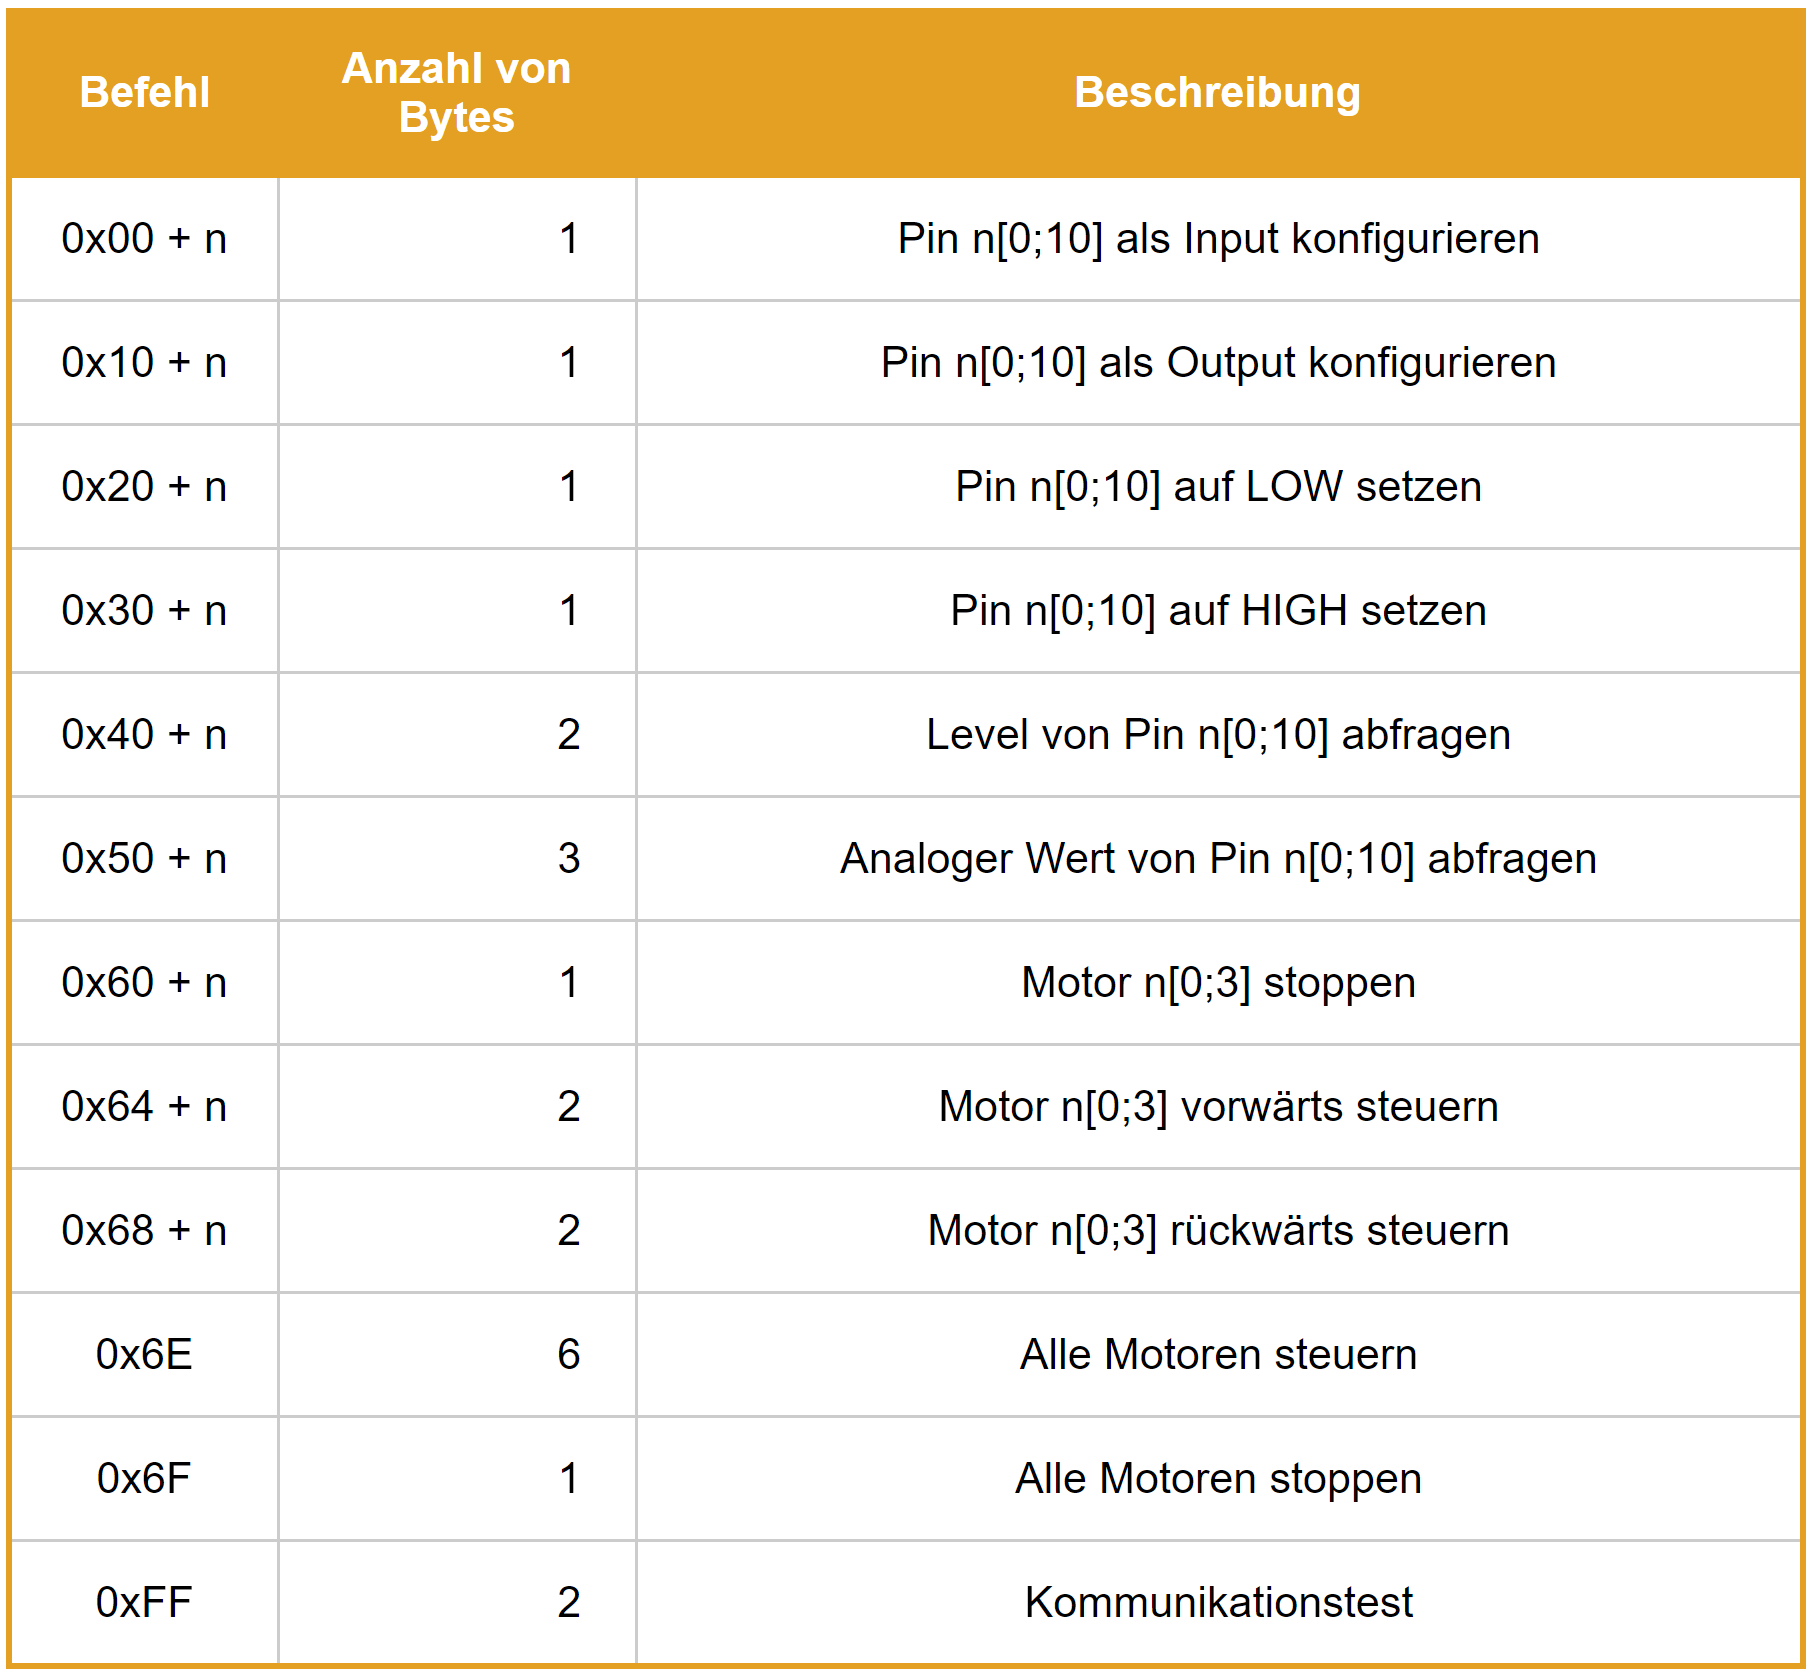
\includegraphics[width=\textwidth]{img/commands.PNG}
\begin{center}\raisebox{9mm}{Abbildung 13: Spezifikation des ATmega-Protokolls (Eigene Darstellung)}\end{center}
Wenn zu Beginn eines Programmes die Funktion \textit{VWAPI.init()} aufgerufen wird, wird die Kommunikation mit dem ATmega überprüft und die Status-LED je nach dem Ergebnis gefärbt. Die Funktion sieht wie folgt aus:
\begin{minted}{c++}
    void init() {
        GPIO(5, GPIO::OUTPUT).setLevel(true);
        GPIO(7, GPIO::OUTPUT).setLevel(true);
        GPIO(17, GPIO::OUTPUT).setLevel(true);
        GPIO(18, GPIO::OUTPUT).setLevel(true);
        GPIO(22, GPIO::OUTPUT).setLevel(true);
        GPIO(27, GPIO::OUTPUT).setLevel(true);

        GPIO(24, GPIO::OUTPUT);
        GPIO(25, GPIO::OUTPUT);

        wait_ms(100);

        SPIDevice mega(22, 0, true, 3000000);
        mega.transfer(0xFF);
        GPIO((mega.transfer(0x00) == 0xAC) ? 24 : 25).setLevel(true);
    }
\end{minted}
\vspace{-2mm}
Zu Beginn werden alle Chip-Select-Pins als Output konfiguriert und auf HIGH gesetzt, danach werden auch die Pins 24 und 25, welche die Status-LED steuern, als Output konfiguriert. Als nächstes wird 100ms gewartet, damit alle Komponenten aktiv sind und keine unerwünschten Probleme am SPI-Bus verursacht werden. Anschließend wird eine Instanz der Klasse \textit{SPIDevice} erstellt und mit dem Chip-Select-Pin 22, SPI-Mode 0 sowie einer Frequenz von 3 MHz konfiguriert. Nun wird der Befehl 0xFF an den ATmega über diese Instanz gesendet. Danach wird ein Byte mit dem Wert 0x00 übertragen und überprüft, ob die Antwort 0xAC entspricht. Sollte dies der Fall sein, wird die grüne LED, welche mit GPIO 24 verbunden ist, eingeschaltet, ansonsten wird die Rote, welche mit GPIO 25 verbunden ist, eingeschalten.
\subsection{IO}
Die IO-Header werden durch den ATmega gesteuert, welcher vom Raspberry Pi die Anweisungen über SPI erhaltet. Jeder IO-Pin kann wie ein GPIO gesteuert werden, jedoch gibt es nur die Modi INPUT und OUTPUT. Die Steuerung der Pins erfolgt über die Klasse \textit{IO}.
\begin{minted}{c++}
#include "SPIDevice.hpp"

class IO {
    char id;
    SPIDevice mega;
public:
    enum Mode {INPUT, OUTPUT = 0x10};
\end{minted}
\vspace{-2mm}
Die Klasse hat zwei Variablen im private-Bereich: \textit{id} speichert die ID des IO-Pins, \textit{mega} ist eine Instanz der Klasse \textit{SPIDevice}, welche zur Kommunikation mit dem ATmega genutzt wird. Zusätzlich dazu definiert die Klasse das Enum \textit{Mode}, welches die beiden Modi der Pins auflistet. Der Import der Klasse \textit{SPIDevice} wird für die SPI-Kommunikation mit dem ATmega benötigt.\\
\begin{minted}{c++}
    IO () {}
\end{minted}
\begin{minted}{c++}
    IO(char id) {
        this->id = id > 8 ? 8 : (id < 1 ? 1 : id);
        this->mega = SPIDevice(22, 0, true, 300000);
    }
\end{minted}
\begin{minted}{c++}
    IO(char id, Mode m) {
        this->id = id > 8 ? 8 : (id < 1 ? 1 : id);
        this->mega = SPIDevice(22, 0, true, 300000);
        setMode(m);
    }
\end{minted}
\vspace{-2mm}
Der Default-Konstruktor ist wie bei vielen anderen Klassen nur zur Erstellung leerer Instanzen gedacht und erfüllt keine spezielle Funktion. \\Die anderen Konstruktor nehmen einen Character beziehungsweise einen Character und ein Objekt vom Typ \textit{Mode} an. Zu Beginn wird die Variable \textit{id} mit dem Wert des ersten Arguments beschrieben, jedoch wird \textit{id }auf das Intervall [1; 8] limitiert. Als nächstes wird eine neue Instanz der Klasse \textit{SPIDevice} erstellt, welche mit dem Chip-Select-Pin 22, SPI Mode 0 und einer Frequenz von 3 MHz konfiguriert wird, bevor sie in der Variable \textit{mega} gespeichert wird. Der Konstruktor, der auch ein Objekt vom Typ \textit{Mode} annimmt ruft die Funktion \textit{setMode} auf, um den Modus des Pins zu setzen.\\
\begin{minted}{c++}
    void setMode(Mode m) {
        this->mega.transfer(m + this->id - 1);
    }
\end{minted}
\begin{minted}{c++}
    void setLevel(bool lvl) {
        this->mega.transfer((lvl ? 0x30 : 0x20) + this->id - 1);
    }
\end{minted}
\vspace{-2mm}
Die Funktion \textit{setMode} dient dazu, den Modus eines IO-Pins zu setzen und nimmt ein Argument vom Typ \textit{Mode} an. Der Modus wird geändert, indem ein bestimmter Befehl über \textit{mega.transfer} gesendet wird. Der Befehl besteht aus einem Byte, welches mit folgender Formel berechnet werden kann:\\cmd = modus + (id - 1), modus ist hierbei 0x00 für einen Input und 0x10 für einen Output.\\\\
Mit der Funktion \textit{setLevel} kann ein Pin, welcher als Output konfiguriert wurde auf HIGH oder LOW gesetzt werden, der Wert wird über eine Boolean übergeben. Auch diese Funktion sendet lediglich ein Byte über SPI, welches folgendermaßen berechnet wird:\\cmd = level + (id - 1), level hat den Wert 0x30 für HIGH und 0x20 für LOW.\\\\
\begin{minted}{c++}
    bool getLevel() {
        mega.transfer(0x40 + this->id - 1);
        return (bool) this->mega.transfer(0x00);
    }
\end{minted}
\vspace{-2mm}
Mit der Funktion \textit{getLevel} kann der Wert eines Input-Pins ausgewertet werden, welcher als Boolean zurückgegeben wird. Die Funktion sendet dazu den Wert 0x40 + (\textit{id} - 1) an den ATmega, danach wird der Wert 0x00 übertragen. Der zweite Rückgabewert wird anschließend in eine Boolean konvertiert und zurückgegeben.
\subsection{ADC}
Ein ADC-Pin ist ein IO-Pin, welcher zusätzlich über den ATmega nicht nur digital, sondern auch analog ausgewertet werden kann. Der Source-Code ist nahezu ident, jedoch wird bei der Berechnung der einzelnen Befehle statt (id - 1) der Term (id + 7) verwendet.\\
\begin{minted}{c++}
#include "SPIDevice.hpp"

class ADC {
    char id;
    SPIDevice mega;
public:
    enum Mode {INPUT, OUTPUT = 0x10};

    ADC() {}

    ADC(char id) {
        this->id = id > 3 ? 3 : (id < 1 ? 1 : id);
        this->mega = SPIDevice(22, 0, true, 1000000);
    }

    ADC(char id, Mode m) {
        this->id = id > 3 ? 3 : (id < 1 ? 1 : id);
        this->mega = SPIDevice(22, 0, true, 1000000);
        this->mega.transfer(m + this->id + 7);
    }
\end{minted}
\begin{minted}{c++}
    void setMode(Mode m) {
        this->mega.transfer(m + this->id + 7);
    }

    void setLevel(bool lvl) {
        this->mega.transfer((lvl ? 0x30 : 0x20) + this->id + 7);
    }

    bool getLevel() {
        mega.transfer(0x40 + this->id + 7);
        return (bool) this->mega.transfer(0x00);
    }
\end{minted}
\begin{minted}{c++}
    unsigned int getAnalog() {
        mega.transfer(0x4F + this->id);
        unsigned int out = ((unsigned int) mega.transfer(0x00)) << 8;
        return out  mega.transfer(0x00);
    }
\end{minted}
\vspace{-2mm}
Alle Funktionen, die auch in der Klasse \textit{IO} existieren, existieren auch in der Klasse \textit{ADC}, jedoch mit der geänderten Berechnung der Befehle, die an den ATmega gesendet werden. Zusätzlich zu den anderen Funktionen gibt es noch die Funktion \textit{getAnalog}, die einen Wert linear zur Spannung des Pins zurückliefert, wobei der Wert 0 für 0 V steht, der Wert 1023 für 5V steht. Dazu wird der Befehl 0x4F + \textit{id} übertragen, bevor zwei Bytes mit dem Wert 0x00 übertragen werden. Der Rückgabewert des ersten Bytes sind die Most-Significant-Bits des Wertes und werden daher zuerst in einen unsigned Integer umgewandelt und anschließend um acht Stellen nach links geschoben, bevor sie in die Variable \textit{out} übertragen werden. Der Rückgabewert des zweiten Bytes sind die acht Least-Significant-Bits, welche einfach mit einem logischen OR zur Variable \textit{out} hinzugefügt werden, bevor jene zurückgeliefert wird.
\subsection{Motor}
Die vier Motor-Outputs werden mit der Klasse \textit{MotorController} gesteuert, womit entweder nur einzelne Motoren oder alle vier Motoren gleichzeitig angesprochen werden können. Die Geschwindigkeit der Motoren wird über ein PWM-Signal kontrolliert, welches der ATmega mit einer Auflösung von acht Bits erzeugt, somit sind 256 Stufen pro Drehrichtung möglich. Die Drehrichtung wird ebenso wie der Duty-Cycle bei der Kommunikation übermittelt und vom ATmega über zwei Pins pro Motor gesteuert.\\
\begin{minted}{c++}
#include "SPIDevice.hpp"

class MotorController {
    SPIDevice mega;
public:
    MotorController() {
        this->mega = SPIDevice(22, 0, true, 1000000);  
    }
\end{minted}
\vspace{-2mm}
Die Klasse \textit{MotorController} definiert nur eine Variable im private-Bereich, welche eine Instanz vom Typ \textit{SPIDevice} ist und zur Kommunikation mit dem ATmega verwendet wird. Der Konstruktor initialisiert diese Variable mit einer neuen Instanz, welche mit dem Chip-Select-Pin 22, SPI Mode 0 und einer SPI-Frequenz von 1 Mhz erstellt wird. Da der Konstruktor keine Argumente benötigt ist somit kein zusätzlicher Default-Konstruktor mehr nötig.\\
\begin{minted}{c++}
    void stopMotor(char motor) {
        motor = motor > 4 ? 4 : (motor < 1 ? 1 : motor);  
        mega.transfer(0x5F + motor);
    }
\end{minted}
\begin{minted}{c++}
    void stopAll() {
        mega.transfer(0x6F); 
    }
\end{minted}
\vspace{-2mm}
Die Funktion \textit{stopMotor} dient zum Stoppen eines Motors, welcher über das erste Argument bestimmt wird. Der Wert des Arguments wird auf den Bereich 1 bis 4 limitiert. Der Befehl zum Stoppen eines Motors wird mit 0x5F + \textit{motor} berechnet und dann an den ATmega übertragen.
Die Funktion \textit{stopAll} stoppt alle Motoren und benötigt somit keine Argumente. Der Befehl zum Stoppen aller Motoren ist 0x6F, daher wird dieser Wert an den ATmega gesendet.\\
\begin{minted}{c++}
    void setMotor(char motor, double speed) {
        motor = motor > 4 ? 4 : (motor < 1 ? 1 : motor);  
        int speed = (speed < -1.0 ? -1.0 : 
            (speed > 1.0 ? 1.0 : speed)) * 255;
        mega.transfer(motor + (speed > 0 ? 0x63 : 0x67));
        mega.transfer(speed < 0 ? (speed * -1) : speed);
    }
\end{minted}
\vspace{-2mm}
Die Funktion \textit{setMotor} nimmt zwei Argumente an, das Erste, welches vom Typ char ist, wählt den Motor-Ausgang, das Zweite bestimmt die Drehgeschwindigkeit als Double. Zuerst wird der gewählte Motor-Ausgang auf das Intervall [1; 4] sowie die Geschwindigkeit auf das Intervall [-1.0; 1.0] beschränkt. Anschließend wird die Geschwindigkeit mit 255 multipliziert und in einen Integer umgewandelt, welcher nun im Intervall [-255; 255] liegt. Danach wird der Befehl an den ATmega gesendet, welcher mit folgender Formel berechnet wird:\\cmd = 0x63 + motor + richtung, wobei motor eine Zahl zwischen 1 und 4 ist und richtung 0 der Richtung vorwärts und 4 der Richtung rückwärts entspricht. Als zweites Byte wird nun der Betrag der Variable \textit{speed} gesendet.\\\\\\
\begin{minted}{c++}
    void setMotors(double m1, double m2, double m3, double m4) {
        char dirs = (m1 > 0 ? 0x80 : 0x40) | (m2 > 0 ? 0x20 : 0x10) |
            (m3 > 0 ? 0x08 : 0x04) | (m4 > 0 ? 0x02 : 0x01);
        int m1s = (m1 < -1.0 ? -1.0 : (m1 > 1.0 ? 1.0 : m1)) * 255;
        int m2s = (m2 < -1.0 ? -1.0 : (m2 > 1.0 ? 1.0 : m2)) * 255;
        int m3s = (m3 < -1.0 ? -1.0 : (m3 > 1.0 ? 1.0 : m3)) * 255;
        int m4s = (m4 < -1.0 ? -1.0 : (m4 > 1.0 ? 1.0 : m4)) * 255;
        mega.transfer(0x6E);
        mega.transfer(m1s < 0 ? (m1s * -1) : m1s);
        mega.transfer(m2s < 0 ? (m2s * -1) : m2s);
        mega.transfer(m3s < 0 ? (m3s * -1) : m3s);
        mega.transfer(m4s < 0 ? (m4s * -1) : m4s);
        mega.transfer(dirs);
    }
\end{minted}
\vspace{-2mm}
Die Funktion \textit{setMotors} dient zum Festlegen der Geschwindigkeit aller vier Motoren und nimmt daher vier Argumente vom Typ Double an. Zuerst wird ein Byte erstellt, welches die Drehrichtung der Motoren speichert, indem wenn Motor 1 sich vorwärts dreht, Bit 7 auf 1 gesetzt wird, ansonsten Bit 6. Für Motor 2 sind die Bits 5 und 4 zuständig, für Motor 3 die Bits 3 und 2 und für Motor 4 die Bits 1 und 0. Anschließend werden die Geschwindigkeiten auf das Intervall [-1.0; 1.0] limitiert und in einen Integer umgewandelt, indem mit 255 multipliziert wird. Nun wird an den ATmega der Befehl 0x6E gesendet, gefolgt von den Beträgen der einzelnen Drehgeschwindigkeiten, welche nach der vorherigen Umrechnung im Intervall [-255; 255] liegen. Als letztes wird das Byte übertragen, in welchem die Drehrichtungen gespeichert sind.\\
\subsection{Externe Komponenten}
Die Verwendung von externen Komponenten ist mit der Library stark vereinfacht, da alle grundlegenden Funktionen vorhanden sind, welche zur Kommunikation oder Steuerung dieser benötigt werden.\\
Zur Bedienung eines Roboters reicht es oft nicht aus, nur einen Ein-Aus-Schalter zu benutzen, daher kann der User-Interface-Header genutzt werden, um Taster, Schalter sowie zusätzliche LEDs mit den Raspberry Pi zu verbinden und diese dann über die Klasse \textit{GPIO} zu steuern. Ein sehr simples Beispielprogramm hierfür wäre folgendes:
\begin{minted}{c++}
#include "VWAPI.hpp"

int main() {
    VWAPI.init();
    GPIO taster(20, GPIO::INPUT);
    GPIO led(21, GPIO::OUTPUT);
    while(true) {
        led.setLevel(taster.getLevel());
    }
}
\end{minted}
\vspace{-2mm}
Dieses Programm setzt eine LED am obersten Pin des User-Interface-Headers (GPIO 21) entsprechend nach dem Status eines Tasters am Pin darunter (GPIO 20). Wichtig ist der Import von \textit{VWAPI.hpp}, damit alle Funktionen und Klassen der Library genutzt werden können. Die Funktion main ist der Einstiegspunkt des Programmes und ruft als erstes die Funktion \textit{VWAPI.init} auf, welche alle Pins richtig initialisiert. Anschließend werden zwei Objekte vom Typ GPIO erstellt, wobei das Erste, \textit{taster}, den Taster steuert und das Zweite, \textit{led}, die LED. Dazu wird der entsprechende Pin sowie der Mode angegeben, der bei der LED Output sowie bei dem Taster Input entspricht. Nun wird mit einer while-Schleife der nächste Teil so lange wiederholt, bis das Board wieder ausgeschaltet wird. Innerhalb  der while-Schleife wird der Pin der LED auf den digitalen Wert des Taster-Pins gesetzt, somit leuchtet die LED nur, wenn auf dem Taster-Pin eine Spannung anliegt, welche für ein logisches HIGH hoch genug ist.
\newpage\section{Fazit}
Alle Entwicklungsschritte von der Platine bis zur fertigen Software wurden wie geplant abgeschlossen und alle Probleme, welche während der Entwicklung aufgetreten sind, konnten erfolgreich behoben werden. Die erste Herausforderung, welche aufgetreten ist, war die Floating-Point-Unit, ohne diese keine Berechnungen mit Gleitkommazahlen durchgeführt werden konnten. Dieses Problem wurde jedoch durch zwei Zeilen im Bootloader behoben, sodass keine weiteren Fehler entstehen können. Zu Beginn der Softwareentwicklung gab es noch keinen Code für UART, somit konnte ich nur über einzelne GPIOs meinen Code debuggen, jedoch hat dies auch ausgereicht. Bei UART musste ich die Baudrate richtig bestimmen, um akkurate Übertragungen zu ermöglichen, was erst durch mein Oszilloskop möglich wurde. Die letzte Challenge war die Kommunikation mit dem ATmega auf ein Minimum an übertragenen Bytes zu reduzieren, diese konnte durch ein sehr kompaktes Protokoll gelöst werden. Das fertige Board werde ich nicht nur bei dem Robotik-Wettbewerb "Robocup Junior" verwenden, sondern auch für andere Projekte, wo ein Controllerboard mit einer hohen Rechenleistung benötigt wird. Dieses Board ist das Resultat von 3 Jahren Erfahrung sammeln, Wissen aneignen und Platinen designen. In der Zukunft werde ich versuchen, den USB-Bus sowie WLAN und Bluetooth auf dem Raspberry Pi Zero W in Bare Metal umzusetzen, da dies einen Upload des Programmes über USB oder sogar WLAN ermöglichen würde. Zusätzlich wäre somit eine Kommunikation zwischen mehreren Raspberry PIs möglich.
\newpage\section{Quellverzeichnis}
\subsection{Literaturverzeichnis}
Atmel Corporation: ATmega644/V. 2012.\\
http://ww1.microchip.com/downloads/en/DeviceDoc/doc2593.pdf $[$Zugriff: 4. 10. 2020$]$\\\\
STMicroelectronics: VNH7100AS. 2016.\\
https://www.st.com/resource/en/datasheet/vnh7100as.pdf $[$Zugriff: 4. 10.2020$]$\\\\
Fairchild: ES3A-ES3J - Fast Rectifiers. 2014.\\
https://datasheet.ciiva.com/4453/es3d-182563-4453353.pdf $[$Zugriff: 7. 10. 2020$]$\\\\
Soininen, Jonne: Linux boot loader and boot in Raspberry Pi. Espoo: 2013.\\
http://softwareji.tistory.com/attachment/cfile3.uf@2415144256962E072E7023.pdf\\
$[$Zugriff: 21. 10. 2020$]$\\\\
Broadcom Corporation: BCM2835 ARM Peripherals. Cambridge: 2012.\\
https://www.raspberrypi.org/app/uploads/2012/02/BCM2835-ARM-Peripherals.pdf\\
$[$Zugriff: 28. 10. 2020$]$
\newpage\subsection{Abbildungsverzeichnis}
Abbildung 1: Eigenes Foto\\
Abbildungen 2 - 13: Eigene Darstellungen\\\\
\section{Abkürzungsverzeichnis}
GPIO... General Purpose Input Output (Pin)\\
VCC... Batteriespannung\\
GND... Ground\\
SPI... Serieller Bus mit vier Leitungen\\
I2C... Serieller Bus mit zwei Leitungen\\
UART... Asynchroner Bus mit zwei Leitungen\\
PWM... Pulsweitenmodulation\\
VFP... Hardware für Gleitkommazahlen\\
ISP... In-System-Programmer
\newpage\section{Source-Code}
Der gesamte Source-Code kann auf meinem GitHub-Account in der Repository \textit{VWA} gefunden werden, welche über folgenden Link erreichbar ist:\\ \hyperlink{https://github.com/NameCeasar/VWA}{https://github.com/NameCeasar/VWA}\\\\
Im Ordner \hyperlink{https://github.com/NameCeasar/VWA/tree/master/SRC}{\textit{SRC}} befindet sich der gesamte Source-Code für das Raspberry Pi, welcher mit Hilfe der Datei \textit{build.bat} kompiliert werden kann. Der Code für den ATmega 644 befindet sich im Ordner \hyperlink{https://github.com/NameCeasar/VWA/tree/master/SRC_ATmega/VWA}{\textit{SRC\_ATmega}}.
\end{document}
